% !TeX root = ../main.tex
\chapter[Assessing and Addressing GPU Memory Safety in the Presence of Data Races]{Assessing and Addressing GPU Memory Safety in the Presence of Data Races}

\section{Personal Context}

\begin{figure}
    \centering
    \captionsetup[subfigure]{width=.45\textwidth}
    \subfloat[Program with a data race on \texttt{i[0]}, which is used to index into \texttt{m}.]{
        \parbox{0.45\textwidth}{
            \centering
            \small
            \begin{tabularx}{\linewidth}{ l | l }
                \multicolumn{2}{l}{\texttt{i: array<u32, 1>, m: array<u32, 4>}} \\
                \midrule
                \multicolumn{1}{c}{\underline{Thread 0}} & \multicolumn{1}{c}{\underline{Thread 1}} \\
                    a: \texttt{i[0] = 2} & c: \texttt{i[0] = 4} \\
                    \ldots \hspace{0.25em} // \texttt{some computation} & \\
                    b: \texttt{let r0 = m[}\textcolor{red}{\texttt{min(}}\texttt{i[0]}\textcolor{red}{\texttt{, 3)}}\texttt{]} & \\
                \midrule
            \end{tabularx}
        }\label{fig:oob-example-a}
    }
    \hfill
    \subfloat[Program with a data race on \texttt{i[0]}, with \texttt{x} used to index into \texttt{m}.]{
        \parbox{0.45\textwidth}{
            \centering
            \small
            \begin{tabularx}{\linewidth}{ l | l }
                \multicolumn{2}{l}{\texttt{i: array<u32, 1>, m: array<u32, 4>}} \\
                \midrule
                \multicolumn{1}{c}{\underline{Thread 0}} & \multicolumn{1}{c}{\underline{Thread 1}} \\
                    a: \texttt{i[0] = 2} & c: \texttt{i[0] = 4} \\
                    \texttt{var x = 2} & \\
                    b: \texttt{let r0 = m[}\textcolor{red}{\texttt{min(}}\texttt{x}\textcolor{red}{\texttt{, 3)}}\texttt{]} & \\
                \midrule
            \end{tabularx}
        }\label{fig:oob-example-b}
    }
    \caption{WGSL compilers insert dynamic bounds-checks (shown in red) to provide memory safety. We show that under current specifications the bounds-checks can be optimized away in either program, leading to potential memory safety violations.}
    \label{fig:oob-example}
    \Description[Programs with bounds checks and data races.]{The first program shows two threads. In the first thread the program writes 2 to i[0], then reads from m[i[3]]. The compiler inserts a min check, in red, around i[3], comparing it to 3, the length of m. The second thread writes 4 to i[0], a data race. The second program is similar except that it uses a private variable x to index into m.}
\end{figure}


\section{Motivation}

\subsection{WGSL Data Race Specification Vulnerability \label{sec:spec-vuln}}

In many languages, e.g., C and C++, data races cause undefined behavior, as they can lead to extremely counterintuitive outcomes. However, because these behaviors are not desirable in security-sensitive contexts (e.g., browsers), languages such as JavaScript and Wasm have defined data races, albeit with very permissive semantics~\cite{weak-wasm, repairing-js}. Similarly, WGSL utilizes compiler passes and safe libraries to avoid many types of undefined behavior. However, the languages which WGSL targets are \textit{not} free of undefined behavior, and in particular follow C/C++ in giving data races undefined behavior. A data race occurs when multiple threads concurrently access the same memory location without proper synchronization. Modern programming languages have adopted special primitives, e.g., \textit{atomic} in C++, and \textit{volatile} in Java, to safely signal when a memory location may be accessed by multiple threads, with their precise semantics defined in formal memory models~\cite{c11, java}.

WGSL derives its memory model from C++, with memory accesses specified as either atomic or non-atomic. \myfiglong{\ref{fig:oob-example-a}} shows a WGSL program with two arrays of unsigned integers, \texttt{i} and \texttt{m}, and two threads performing non-atomic accesses to these arrays. This program contains behaviors that, in isolation, are undefined in some languages: (1)~because memory locations are non-atomic and there is no synchronization, there are data races between ($a$, $c$) and ($b$, $c$), and (2)~while the race technically makes the program undefined, a possible natural compilation could allow for an out-of-bounds read if $b$ reads the value $c$ wrote to \texttt{i[0]}. The potential out-of-bounds read is a memory safety violation which, in turn, could lead to a vulnerability. The highlighted code in operation $b$, i.e.,\xspace \textcolor{red}{\texttt{min(..., 3)}}, shows a check that WGSL compilers include to enforce memory safety. However, WGSL compilers currently contain no special protections against data races.

\paragraph{The Problem: Optimizing Away Bounds-Checks} Even with the bounds-check inserted, a compiler for an unsafe lower-level language can optimize the code in a way that inserts a ``time-of-check to time-of-use'' (TOCTOU)~\cite{abbott1976toctou} memory safety violation. Specifically, a compiler for an unsafe language is free to assume programs do not contain data races. Therefore, when only looking at the operations in thread 0, the compiler may notice that \texttt{i[0]} is set to 2 and remains unchanged until it is loaded in $b$. Based on a range analysis, it can determine that the call to \texttt{min} is unnecessary and remove it, leading to an out-of-bounds access if \texttt{i[0]} reads 4 in $b$. While it is unlikely a real implementation would perform the problematic optimization on this particular program, in \mysec\ref{sec:extended-example} we describe a more realistic program that could trigger this optimization.

The program in \myfig\ref{fig:oob-example-a} shows straightforwardly how data races can lead to vulnerabilities, but memory safety issues can occur due to other surprising behaviors allowed by data races. In particular, \myfig\ref{fig:oob-example-b} shows a WGSL program which contains the same data race between $a$ and $c$, but now the access to \texttt{m} in $c$ depends on a separate variable \texttt{x}. Prior work shows how reasonable implementations might set \texttt{x} to 4--for example if the compiler notices that both \texttt{x} and \texttt{i[0]} contain the same value (2), and decides to not allocate a register for \texttt{x}, reloading \texttt{i[0]} instead and causing a potential out-of-bounds access~\cite{bounding-races}.

To recap, WGSL code, i.e., \myfig\ref{fig:oob-example} without the \textcolor{red}{\texttt{min}}, is written by application developers, and may contain out-of-bounds accesses and data races. To avoid out-of-bounds accesses, WGSL compilers insert bounds-checks when generating lower-level native GPU code. The WGSL specification also mandates that if a data race occurs, memory accesses should be restricted to in-bounds memory in order to maintain memory safety~\cite[\mysec 2.2]{wgslspec}, but WGSL compilers do not include any special protections against data races. However, native GPU languages currently give undefined semantics to data races, allowing the optimizations described above when compiling to vendor-specific machine code. This mismatch between the WGSL specification and the native language guarantees means that the bounds-checks can be removed despite the fact that they should not be to maintain memory safety, creating the WGSL DRSV.

\paragraph{The Solution: Constraining Optimizations}

The optimizations described above must be disallowed so that the bounds-checks remain, i.e., to maintain memory safety. In \myfig\ref{fig:oob-example-a}, this can be achieved by specifying that all accesses to \texttt{i[0]} be \textit{atomic}. Atomic accesses signal to the compiler that multiple threads might modify \texttt{i[0]}, preventing it from making the assumption that \texttt{i[0]} remains unchanged between $a$ and $b$. In \myfig\ref{fig:oob-example-b}, the compiler must be prevented from using the value in \texttt{i[0]} to refer to \texttt{x}. While this could be accomplished by again making accesses to \texttt{i[0]} atomic, extending this principle to full programs would require making \textit{every} memory access atomic, causing unacceptable performance decreases for many applications. Rather, we propose two properties which ensure memory safety violations do not occur due to data races while making a minimal set of accesses atomic. We call these properties the \saferace Memory Safety Guarantee (\smsg).

The first property of \smsg specifies that slices of programs which contribute to memory indexing must be race-free, and can be applied in \myfig\ref{fig:oob-example-a} by making accesses to \texttt{i[0]} atomic. In more complex code, multiple accesses may contribute to the calculation of the index into \texttt{m}. In these cases, it is not necessary to do the complete index calculation atomically, i.e., by loading all memory and performing arithmetic indivisibly. Rather, it is sufficient to ensure that each sub-access which contributes to the calculation is done atomically, using a backward slicing algorithm which considers all control, index, and data dependencies of an access. In \mysec\ref{sec:saferace}, we show formally how this avoids data races on the full index calculation and ensures memory safety.

The second property of \smsg specifies that data races cannot affect the behavior of race-free program slices, preventing the data race on \texttt{i[0]} from affecting the index into \texttt{m} in \myfig\ref{fig:oob-example-b}. The first property can be implemented as a compiler pass, while the second property must be adopted by intermediate representations which WGSL targets. In \mysec\ref{sec:saferace} we formally define both properties, and in \mysec\ref{sec:smsg-prop-1} and \mysec\ref{sec:smsg-prop-2} we evaluate the performance and practical impacts of adopting them.

\subsection{\saferace: Threat Assessments and Specification Proposals}

Given the potential for attackers to exploit the specification vulnerability outlined above, we present \saferace, a thorough investigation into how data races can affect memory safety properties when compiling WGSL (a safe language) to lower-level unsafe languages. We perform threat assessments that test native frameworks and WebGPU implementations for memory isolation vulnerabilities and introduce specification proposals which ensure WGSL's memory safety in the presence of data races. Our results provide a framework which can inform the development of other languages with similar compositional designs.

\paragraph{Threat Assessment: Bottom-Up (\mysec\ref{sec:assess-bu})}
First, we assess the potential for programs with simple memory safety violations, e.g., out-of-bounds accesses without bounds-checks, to cause vulnerabilities.
%The results of this study highlight how straightforwardly memory safety violations can be exploited to memory isolation vulnerabilities for GPUs.
We conduct our assessment in two native GPU frameworks: Vulkan, which runs on Linux and Android operating systems, and Metal, which runs on macOS and iOS.
%Our assessment targets the main classes of memory used in general-purpose GPU programs, each which have differing hardware implementations. Additionally, we run our assessment in two modes as a malicious WGSL program might try to access memory from another tab in the browser (same-process mode) or from a different program running on the host (different-process mode).
We test 11 GPUs from 6 vendors and discover two new memory isolation vulnerabilities, one due to uninitialized memory on AMD GPUs and the other due to out-of-bounds accesses on Apple GPUs.

\paragraph{Threat Assessment: Top-Down (\mysec\ref{sec:assess-td})}
We develop a fuzzer, \wgslmemsmith, based on WGSLSmith~\cite{lecoeur2023reconditioning}, to test WGSL implementations for the \drsv, i.e., the data race specification vulnerability described above. \wgslmemsmith generates random programs that contain potential memory safety violations due to combinations of data races and out-of-bounds accesses in order to determine whether WGSL's \drsv can be triggered by existing compilers. We run \wgslmemsmith on 21 unique compilation stacks, i.e., combination of browser, operating system, and GPU vendor, and show that the specification vulnerability is either not implemented or is unlikely to be triggered.

Despite our negative result, the vulnerability remains a ticking time bomb, motivating the development of the specification proposals introduced below. Additionally, our fuzzing finds a simpler memory isolation vulnerability due to missing bounds-checks in a pre-release version of Firefox; this vulnerability has been confirmed and fixed by Mozilla developers. %Finally, to raise confidence in our testing approach, we conduct mutation testing on our fuzzer and analyze the characteristics, e.g., register pressure, of the generated programs.

\paragraph{\saferace Memory Safety Guarantee (\mysec\ref{sec:saferace})}
To fix the WGSL \drsv, we introduce the \saferace Memory Safety Guarantee (\smsg), a contract between a higher-level memory-safe language and lower-level unsafe languages. \smsg consists of two properties: (1)~program slices which contribute to memory indexing, e.g., events $a$, $b$, and $c$ in \myfig\ref{fig:oob-example-a}, must be race-free, and (2)~data races cannot affect the behavior of race-free slices of programs. %In \mysec\ref{sec:sr-reasoning}, we formally define how to construct program slices.

%for a memory access $A$, all shared memory accesses which contribute to the memory locations accessed by $A$, e.g., \texttt{i[0]} in $b$ in \myfig\ref{fig:oob-example}, cannot themselves take part in a data race, and (2)~a data race on an unrelated memory access $A'$ cannot affect the behaviors of $A$. Note that the second property entails that data races are no longer considered globally undefined behavior.

Property 1 can be enforced by an initial pass in WGSL compilers which ensures a program slice is race-free by translating some non-atomic memory accesses into atomic accesses.  We implement Property 1 in Tint, the compiler for WGSL programs included in Chromium-based browsers. Some data types in WGSL, e.g., floats, cannot currently be accessed atomically, so our implementation cannot apply to all possible WGSL programs, e.g., a program with a conditional on floating point values to determine the index into a memory region. However, our experimental results (\mysec\ref{sec:smsg-prop-1}) show that for a set of important benchmarks, no data types which cannot be accessed atomically are affected by Property 1. We also show that Property 1 has negligible performance impact on many existing WebGPU applications, including AI inference and general compute applications, with the only observed impact being a 10\% performance overhead in a sorting GPU kernel. Property 2 ensures that data races do not affect race-free slices of programs and must be incorporated into the frameworks targeted by WGSL, i.e., currently Vulkan, Metal, and DirectX. We augment \wgslmemsmith with the ability to perform metamorphic fuzzing between programs with and without data races and find violations of Property 2 on only one (likely buggy) machine, providing evidence that these frameworks could relatively straightforwardly adopt this constraint (\mysec\ref{sec:smsg-prop-2}).

\paragraph{Applications Beyond WebGPU (\mysec\ref{sec:broader-impacts})}

While the main body of this work focuses on WGSL, the ideas expressed in our threat assessments and specification proposals apply to other parallel programming languages. An increasing number of modern languages are being developed that strive to maintain memory safety through combinations of features like bounds-checked accesses and ownership of data. At the same time, there is a proliferation of tools that can transpile one language to another, and new processors and accelerators with diverse architectures are being developed. This increases the likelihood that layered compilation stacks will become more prevalent, where safety properties must be evaluated across source and target languages.


\subsection{Contributions}

In summary, our contributions are:

\begin{itemize}
    \item A bottom-up threat assessment that shows memory safety violations can straightforwardly lead to memory isolation failures in many GPU frameworks; resulting in the discovery of two new GPU isolation vulnerabilities (\mysec\ref{sec:assess-bu}).
    \item A top-down threat assessment using \wgslmemsmith to evaluate whether the WGSL \drsv is currently exploitable. We show that the \drsv is likely \textit{not} exploitable today, while also discovering a memory isolation vulnerability in a pre-release version of Firefox (\mysec\ref{sec:assess-td}).
    \item The \saferace Memory Safety Guarantee (\smsg), two properties that when combined provide memory safety in the presence of data races in WGSL programs (\mysec\ref{sec:saferace}).
    \item An implementation of \smsg Property 1 as a WGSL compiler pass and an evaluation that shows it negligibly impacts the performance of a set of WebGPU applications (\mysec\ref{sec:smsg-prop-1}).
    \item A metamorphic fuzzing approach implemented in \wgslmemsmith which finds that \smsg Property 2 is empirically supported by most systems we tested (\mysec\ref{sec:smsg-prop-2}).
    %\item A discussion of how our techniques can inform the development of other security-conscious parallel programming frameworks (\mysec\ref{sec:broader-impacts}).
\end{itemize}

\noindent
Our artifact for this work is publicly available~\cite{levine2025saferaceartifact}. As part of responsible disclosure, we have presented this work to the W3C WebGPU working group and reported our vulnerabilities to the affected vendors.

\begin{table}
\scriptsize
\centering
\caption{Results from our bottom-up threat assessment. We find two new vulnerabilities, highlighted in red, both which affect memory isolation when applications are run in different processes.} %Memory isolation is typically not guaranteed when applications are run in the same process, so browsers executing GPU tasks in this configuration must avoid vulnerabilities from occurring through bounds checks and other precautions.}
\begin{tabularx}{.95\linewidth}{ l l l l l l l l l l }
\toprule
& & & \textbf{Memory Region:} & \multicolumn{2}{c}{\textbf{Device}} & \multicolumn{2}{c}{\textbf{Phys. Storage}} & \multicolumn{2}{c}{\textbf{Workgroup}} \\
\cmidrule(lr){5-6} \cmidrule(lr){7-8} \cmidrule(lr){9-10}
\textbf{Framework} & \textbf{OS} & \textbf{Device} & \textbf{Process:} & \textit{same} & \textit{diff} & \textit{same} & \textit{diff} & \textit{same} & \textit{diff} \\
\midrule
\multirow{7}{*}{Vulkan} & \multirow{5}{*}{Linux}   & AMD Radeon RX 7900 XT    & & \cmark  & \cmark                    & \oob    & \cmark & \uninit      & \uninit \\
                        &                          & AMD Ryzen 7 5700G        & & \uninit & \textcolor{red}{\uninit}  & \oob    & \cmark & \cmark       & \cmark  \\
                        &                          & Intel Arc A770 Graphics  & & \cmark  & \cmark                    & \oob    & \cmark & \cmark       & \cmark  \\
                        &                          & Intel UHD Graphics 770   & & \cmark  & \cmark                    & \oob    & \cmark & \cmark       & \cmark  \\
                        &                          & NVIDIA GeForce RTX 4070  & & \cmark  & \cmark                    & \oob    & \cmark & \oob/\uninit & \cmark  \\
\cmidrule(lr){2-10}
                        & \multirow{3}{*}{Android} & Arm Mali-G710            & & \uninit & \cmark                    & \uninit & \cmark & \cmark       & \cmark  \\
                        &                          & Qualcomm Adreno 610      & & \cmark  & \cmark                    & \NA     & \NA    & \uninit      & \cmark  \\
                        &                          & Qualcomm Adreno 740      & & \cmark  & \cmark                    & \NA     & \NA    & \cmark       & \uninit \\
\midrule
\multirow{3}{*}{Metal}  & \multirow{3}{*}{macOS}     & Intel Iris Plus Graphics & & \cmark & \cmark                     & \NA     & \NA    & \cmark       & \cmark  \\
                        &                          & Apple M2                 & & \oob   & \textcolor{red}{\oob}      & \NA     & \NA    & \uninit      & \uninit \\
                        &                          & Apple M3                 & & \oob   & \cmark                     & \NA     & \NA    & \cmark       & \cmark  \\
\bottomrule
\multicolumn{10}{l}
{\cmark = No Vulnerability \oob = Out-of-bounds Access Vulnerability \uninit = Uninitialized Memory Vulnerability} \\
\end{tabularx}
\label{tab:study-results}
\end{table}

\section{Threat Assessment: Bottom-Up \label{sec:assess-bu}}

We first motivate memory safety in WGSL by performing a bottom-up threat assessment; that is, we aim to explore whether memory safety violations lead to memory isolation vulnerabilities in WGSL target languages. As GPUs can be utilized by multiple concurrent processes on the same machine, any memory isolation failure that leaks data between processes is cause for concern.
%and must be addressed as a serious vulnerability by vendors.

%We do not currently have code that targets DirectX, as this framework provides strong memory isolation guarantees by default. Additionally, we do not test iOS devices due to the lack of developer support in iOS for running multiple GPU compute processes concurrently.

Our assessment covers two frameworks and three operating systems, Vulkan (Linux and Android) and Metal (macOS), as well as three address spaces exposed by WebGPU: device, workgroup, and private memory. Since many browsers run WGSL programs from different tabs on the same process, we test for memory isolation both when GPU programs are running in different processes and in the same process. This assessment runs two programs concurrently---a victim and an attacker---and tests for memory isolation failures due to uninitialized memory and out-of-bounds accesses.

The victim allocates a block of memory, with the size dependent on the type of memory being tested. Then, the victim launches many GPU threads, with each thread assigned a set of memory locations within the block of memory. Each thread alternately writes a canary value and a secret value to even and odd memory locations, respectively. Writing a canary allows us to avoid false positives where the attacker spuriously reads the secret value and tests whether the attacker is able to read consecutive out-of-bounds memory values. The victim's memory is continually re-allocated, either automatically in the case of private and workgroup memory or manually in the case of device memory. The victim runs indefinitely until manually stopped.

Like the victim, the attacker allocates a block of memory, and assigns each thread a set of memory locations. However, the memory locations assigned to each thread of the attacker may be either in or out-of-bounds of the allocated block of memory. The attacker threads iterate over their assigned memory locations and search for the canary, which if found in-bounds indicates that the allocated memory was previously used by the victim and not cleared properly, or if found out-of-bounds indicates that the attacker is able to read real data outside its allocated block. If the canary is found, the attacker records the value of the next memory location and the results are analyzed to determine whether the secret value was found.

Generally, GPU memory references cannot be manipulated using integer arithmetic, e.g., like pointers in C-like languages, which restricts the ability to write certain algorithms, e.g., arbitrary tree structures. However, Vulkan has introduced a new type of memory, \textit{physical storage buffers}, allowing applications to pass a virtual 64-bit address directly to a shader that can be dereferenced and manipulated similarly to a pointer. The memory safety implications of physical storage buffers is not well understood, so we assess both device memory using traditional buffer bindings and physical storage buffers in Vulkan.


\subsection{Evaluation \label{sec:assess-bu-eval}}

\mytablong\ref{tab:study-results} shows the results of our threat assessment. Overall, we test 11 GPUs from 6 vendors using 2 frameworks and 3 operating systems. Every GPU except the Intel devices show a memory isolation failure. %We discovered two vulnerabilities in the different-process mode: one due to uninitialized memory on AMD integrated GPUs and the other due to out-of-bounds accesses on Apple M2 GPUs. These vulnerabilities are highlighted in red in \mytab{\ref{tab:study-results}}. Other vulnerabilities reported in the table were either found in previous work or are in the same-process mode, which is known to have fewer security guarantees but remains concerning due to the runtime configuration of browsers.
We do not show results from private memory, as we observed no failures in this region.

\subsubsection{Same-Process Mode\label{sec:sp-config}}

This mode follows the setup in many browsers, where GPU programs are run in the same process. Failures observed in this mode are not considered vulnerabilities by vendors, as memory isolation is not guaranteed between applications in the same process. However, in the browser these failures would allow an attacker to read data from another tab if bounds-checks were optimized away, highlighting the danger posed by WGSL's specification vulnerability.

Both the AMD Ryzen 7 5700G, an integrated GPU, and the Arm Mali-G710, a mobile GPU, had uninitialized device memory isolation failures, while the Apple M2/M3 GPUs had out-of-bounds access isolation failures. Every device we tested that supports physical storage buffers also had failures. While WebGPU does not support physical storage buffers, our results underscore the need for caution when adopting new GPU features. In workgroup memory, the AMD Radeon RX 7900 XT, NVIDIA GeForce RTX 4070, Qualcomm Adreno 710, and Apple M2 had failures. Memory isolation failures due to uninitialized workgroup memory was reported by prior work~\cite{leftover-locals}, which ran tests in a different-process mode. Our results show that some GPUs which are susceptible to this attack in the different-process mode also are susceptible in the same-process mode. The NVIDIA GPU is the only device which had failures due to out-of-bounds accesses in workgroup memory.

%All vulnerabilities are potential security threats, but out-of-bounds accesses are perhaps more concerning; an attacker can leak memory while a victim process is still running, stopping victims from avoiding leaks by clearing memory at the end of execution. Our results show that Apple GPUs and the NVIDIA GPU are vulnerable to out-of-bounds access violations in the same-process mode.

%On their own, the vulnerabilities found in the same-process mode are not considered serious because generally, fewer security guarantees are afforded to applications running in the same process. However, our results show that if WebGPU's protections against undefined behavior were to be defeated, a wide range of GPUs would leak data to attackers. This further motivates the development of the \wgslmemsmith fuzzer and the strengthening of GPU specifications to mitigate the effects of undefined behavior.

\subsubsection{Different-Process Mode\label{sec:df-config}}

We also test memory isolation of GPU frameworks in a different-process mode, as an attacker running code from the browser might also attempt to steal data from other applications running on the same machine. %for two reasons: (1) memory isolation vulnerabilities across process boundaries are considered to be a serious vulnerability, and (2) the results allow implementers to understand the safety properties of native frameworks when deciding how to set up runtimes.
In device memory, we observe failures on two GPUs: the AMD Ryzen 7 5700G and the Apple M2. These failures can be exploited by a malicious process on the same machine to leak data from victim applications or construct covert channels. We describe each of these vulnerabilities below. Additionally, we observe uninitialized workgroup memory isolation failures on the AMD Radeon RX 7900 XT, Qualcomm Adreno 740, and Apple M2, replicating results from previous work~\cite{leftover-locals}.

\paragraph{AMD Uninitialized Memory Vulnerability}

This vulnerability allows an attacker to read uninitialized memory which can contain data written from another process, if the attacker uses AMD's open-source Mesa drivers. We confirmed that multiple AMD-integrated GPUs are affected, both the Ryzen 7 5700G in our study and a Ryzen 5 5600H. This vulnerability was confirmed by AMD, assigned a CVE~\cite{CVE-2024-36353}, and a patch for the AMD drivers was released.% Even without vendor mitigations, applications can protect against this vulnerability by clearing memory at the end of execution, as this vulnerability only occurs when an attacker is allocated memory that previously belonged to a different process.

\paragraph{Apple M2 Out-Of-Bounds Access Vulnerability}

This vulnerability allows an attacker to access data from another process by performing out-of-bounds accesses. The extent of this vulnerability is limited---only reliably leaking one 32-bit value before driver or hardware protections seemed to kick in (perhaps in response to a previous vulnerability that allowed arbitrary access to out-of-bounds memory~\cite{nist_cve_2022_32947}). Nevertheless, we show that the remaining vulnerability is enough to construct a reliable (albeit slow) covert channel between two processes. This vulnerability, which affects Apple M1 and M2 GPUs, has been reported to and confirmed by Apple.

\lstset{
    language=C,
    basicstyle=\ttfamily\small,
    keywordstyle=\color{blue},
    commentstyle=\color{mygray},
    stringstyle=\color{red},
    showstringspaces=false,
    numbers=left,
    numberstyle=\tiny\color{mygray},
    stepnumber=1,
    numbersep=5pt,
    backgroundcolor=\color{white},
    frame=single,
    captionpos=b,
    morekeywords={restrict},
    moredelim=[is][\textcolor{red}]{@}{@}  % Set delimiter to change color
}

\begin{figure}[t]
    \centering
    \begin{lstlisting}[caption={Extension of \myfig\ref{fig:oob-example} showing a C program which exemplifies WGSL's data race specification vulnerability. Pointers are restricted to avoid aliasing, as in WGSL.}, label={list:c-code}, basicstyle=\small, xleftmargin=10pt, xrightmargin=10pt]
@int min(int a,int b) {return (b<a)?b:a;}@

void f(int *restrict idx, int *restrict data, int *restrict output) {
    if (*data == 0)
        *idx = 17;
    else
        *idx = 19;
    if (*idx < 100)
        *output = data[@min(@*idx, @99)@];
}
    \end{lstlisting}
     \Description[Program showing WGSL's DRSV]{A C++ function with three arguments as restricted int pointers, idx, data, and output. If the value of data is 0, writes 17 to idx, otherwise writes 19. Then, if idx is less than 100, sets output to data[idx]. The compiler inserts a min check comparing idx to 99.}
\end{figure}

\lstset{
    language=LLVM,
    basicstyle=\ttfamily\small,
    morekeywords={align},
    keywords=[2]{i32, i64},
    keywordstyle=[2]\color{purple},
    showstringspaces=false,
    numbers=left,
    numberstyle=\tiny\color{mygray},
    stepnumber=1,
    numbersep=5pt,
    backgroundcolor=\color{white},
    frame=single,
    captionpos=b,
    moredelim=[is][\textcolor{orange}]{@}{@}  % Set delimiter to change color
}

\begin{figure}[t]
    \centering
    \begin{lstlisting}[caption={Compiler optimizations can turn the code in \mylisting\ref{list:c-code} into this LLVM intermediate representation.}, label={list:llvm-code}, xleftmargin=10pt, xrightmargin=10pt]
  %data_0 = load i32, ptr %data, align 4
  %data_is_0 = icmp eq i32 %data_0, 0
  @%idx_0@ = select i1 %data_is_0, i32 17, i32 19
  store i32 @%idx_0@, ptr %idx, align 4
  @%idx_0_ext@ = zext nneg i32 @%idx_0@ to i64
  @%data_ptr@ = getelementptr inbounds i32, ptr %data, i64 @%idx_0_ext@
  %data_val = load i32, ptr @%data_ptr@, align 4
  store i32 %data_val, ptr %output, align 4
    \end{lstlisting}
    \Description[LLVM code]{The LLVM representation of the listing above compiled using some specific passes}
\end{figure}

\section{Threat Assessment: Top-Down \label{sec:assess-td}}

Our top-down threat assessment aims to determine whether the WGSL data race specification vulnerability (\drsv) is exploitable today. We perform this assessment through a large-scale fuzzing campaign with \wgslmemsmith, an extension of the WGSLSmith fuzzer~\cite{lecoeur2023reconditioning} which we developed. The design of \wgslmemsmith is informed by understanding how compilers might optimize away bounds-checks like the one in \myfig\ref{fig:oob-example}. Therefore, we first extend the example from \myfig\ref{fig:oob-example} to examine how valid compiler passes in real implementations might introduce memory safety violations, then show how \wgslmemsmith generates \textit{patterns} which could trigger the specification vulnerability.
%\wgslmemsmith implements a \textit{metamorphic} fuzzing strategy~\cite{chen1998metamorphic}, comparing the outputs from a \textit{safe shader}, i.e., one without data races or other sources of undefined behavior, and a racy shader.
%Racy shaders include data races and patterns similar to the examples in \myfig\ref{fig:oob-example} and \mylisting\ref{list:c-code} to test whether memory isolation vulnerabilities can occur.


\subsection{Extended Example \label{sec:extended-example}}

\mylistinglong\ref{list:c-code} shows C code that implements the same out-of-bounds protections as the GPU example in \myfig\ref{fig:oob-example}. We use C here because it allows us to utilize the LLVM compiler project to easily explore optimization passes. In contrast, optimizing compilers for GPUs are either closed source or don't provide tools that allow fine-grained control of optimizations in an easily configurable way. Also, while there are differences in intermediate representations built specifically for GPUs, the concepts necessary to understand the specification vulnerability in WGSL can be explored in LLVM. %and in fact many GPU vendors have LLVM backends for their hardware~\cite{Faith2022NIR}.

In this example, assume that the length of the \texttt{data} array is 100. The code in red, i.e., the \textcolor{red}{\texttt{min}} check, would be added by a compiler for a memory-safe language. The rest of the code would be written by an application developer (in the memory-safe language). In a single-threaded context, there is no possibility of an out-of-bounds access in this code, but in code running on a parallel processor a separate thread might create a data race on \texttt{*idx}, writing a value greater than 99.


The LLVM code in \mylisting{\ref{list:llvm-code}} shows the results of emitting LLVM from the C code using \texttt{clang} and running the following LLVM optimization passes using \texttt{opt}: \texttt{inline}, \texttt{mem2reg}, \texttt{early-cse}, \texttt{instcombine}, and \texttt{simplifycfg}. In the resulting code, a register \textcolor{orange}{\texttt{\%idx\_0}} is allocated that holds the results of the conditional check on the value of \texttt{ptr \%data} (\mylisting\ref{list:llvm-code} lines 1-3), which corresponds to the conditional on \texttt{data} in \mylisting\ref{list:c-code} lines 4-7. The value of \textcolor{orange}{\texttt{\%idx\_0}} is stored to \texttt{ptr \%idx} (\mylisting\ref{list:llvm-code} line 4), which corresponds to the two stores to \texttt{idx} in \mylisting\ref{list:c-code} lines 5 and 7. Instead of reloading the value of \texttt{ptr \%idx}, the value of \textcolor{orange}{\texttt{\%idx\_0}} is used (extended to an \texttt{i64}) to index into \texttt{ptr \%data} since the compiler assumes the value of \texttt{ptr \%idx} has not changed (\mylisting\ref{list:llvm-code} lines 5-6). This also allows the compiler to provably remove the \textcolor{red}{\texttt{min}} check in \mylisting\ref{list:c-code} line 9 when loading from \texttt{ptr \%data\_ptr} (\mylisting\ref{list:llvm-code} line 7). Note that the conditional in \mylisting\ref{list:c-code} line 8 is also optimized away in \mylisting\ref{list:llvm-code}.

%\footnote{The LLVM code here also includes the \texttt{inbounds} keyword, which specifies that \texttt{ptr \%7} is \texttt{poison} if the offset address is out-of-bounds. As many GPU vendors internally use IRs based on LLVM, we speculate that better handling of \texttt{poison} values by GPU compilers may help avoid the memory isolation violations we find in this paper.}.

In this example, the compiled code is still safe, as the compiler uses \textcolor{orange}{\texttt{\%idx\_0}} instead of loading from \texttt{ptr \%idx}. However, in a more complex program, extra computation could cause register pressure, leading to \textcolor{orange}{\texttt{\%idx\_0}} being spilled to memory before being used to index into \texttt{ptr \%data}. A valid optimization could then rematerialize \textcolor{orange}{\texttt{\%idx\_0}} from \texttt{ptr \%idx}, saving a stack slot\footnote{This same optimization was shown to be problematic when bounding certain data race behaviors in prior work~\cite{bounding-races}.}. Given a data race on \texttt{ptr \%idx}, this value might be larger than the size of \texttt{data}, causing an out-of-bounds access. As far as we know, this optimization is not in LLVM, although it has been proposed~\cite{llvm_memory_use_markers}. This exploration shows that if the \drsv in WGSL is exploitable, it is likely due to programs that are susceptible to these types of optimizations. We now describe the base shaders \wgslmemsmith generates and then show how patterns which might trigger these optimizations are incorporated into the shaders.

%This same optimization was shown to be the potential cause of data races not being bound in space. Similar to how we modified \myfig\ref{fig:oob-example}, we could change line 14 of \mylisting\ref{list:c-code} to use some other variable \texttt{x} as the index into \texttt{data} and in the presence of data races cause a compiler to generate unsafe code.

\begin{figure}
    \small
    \centering
    \captionsetup[subfigure]{width=.32\textwidth}
    \subfloat[Basic Pattern. Thread 1 races on \texttt{i[0]}, writing an out-of-bounds value, e.g., 4.\label{fig:basic-pattern}]{
        \parbox{0.32\textwidth}{
            \centering
            \begin{tabularx}{.8\linewidth}{ l }
                \midrule
                \underline{Thread 0} \\
                \texttt{a: i[0] = 2} \\
                \texttt{b: }\textcolor{blue}{\texttt{let}}\texttt{ r0 = m[i[0]]} \\
                \midrule
            \end{tabularx}
        }
    }
    \hfill
    \subfloat[Undefined Arithmetic Pattern. Thread 1 writes a value that causes overflow, e.g., 2 billion.\label{fig:arith-pattern}]{
        \parbox{0.32\textwidth}{
            \centering
            \begin{tabularx}{.8\linewidth}{ l }
                \midrule
                \underline{Thread 0} \\
                \texttt{i[0] = 500000} \\
                \textcolor{blue}{\texttt{let}}\texttt{ r0 = m[1 + i[0]]} \\
                \midrule
            \end{tabularx}
        }
    }
    \hfill
    \subfloat[Control-Flow Pattern. Thread 1 writes a value that causes the conditional to execute, e.g., 1.\label{fig:control-pattern}]{
        \parbox{0.32\textwidth}{
            \centering
            \begin{tabularx}{.8\linewidth}{ l }
                \midrule
                \underline{Thread 0} \\
                \texttt{i[0] = 0} \\
                \textcolor{blue}{\texttt{var}}\texttt{ x = 0} \\
                \textcolor{blue}{\texttt{if}}\texttt{ (i[0] > 0) x = 4 } \\
                \textcolor{blue}{\texttt{let}}\texttt{ r0 = m[x]} \\
                \midrule
            \end{tabularx}
        }
    }
    \caption{The three types of patterns that \wgslmemsmith generates. Here, \texttt{i} is a signed 32-bit integer array of size 1 and \texttt{m} is an unsigned 32-bit integer array of size 4 in either device, workgroup, or private memory.}
    \Description[Pattern code]{Each of the three tables shows the different types of patterns.}
    \label{fig:patterns}
\end{figure}


\subsection{Shader Generation \label{sec:base-gen}}

\wgslmemsmith generates shaders in a single pass. It currently supports a subset of WGSL types and expressions, consisting of assignment statements, integer arithmetic, conditionals, and loops. %Memory locations are split into \textit{safe} and \textit{unsafe} sets. Safe memory locations do not participate in data races, while unsafe memory locations may be affected by data races.
%Safe global memory locations are read-only, while unsafe global memory locations may be read or written to by any thread. Similarly, safe thread memory locations are guaranteed to be read and written by only one thread, while unsafe thread memory locations may be read or written by other threads. Safe local variables are only used in combination with safe memory locations, while unsafe variables can be combined in expressions with unsafe memory locations.
Assignment statements have a variable number of operands in their expressions---by default between 1-3. Optionally, a setting \textit{register pressure} can be turned on, which increases the number of operands in expressions (up to 20) and prioritizes using local variables in order to increase the number of registers the compiler might allocate. Overall, there are 16 parameters when generating shaders that can be modified at runtime. This allows us to run comprehensive fuzzing campaigns that randomly generate shaders with different parameters at each iteration.

%First the safe shader is run and the resulting (deterministic) memory values are saved. Next, the racy shader, which contains the statements in the safe shader along with statements that operate on unsafe memory locations and may contain data races, is run. The values in safe memory locations at the end of the racy shader execution are compared with the values from the safe shader execution. Because safe and unsafe locations are completely disjoint, differing values may have been caused by data races, violating \smsg Property 2 .

%\subsection{Pattern Generation \label{sec:pattern-gen}}

Along with the base shader, \wgslmemsmith generates racy \textit{patterns} that seek to induce compiler optimizations that could trigger the WGSL \drsv. Patterns are based on templates instantiated during the generation process, with the three types of patterns shown in \myfig\ref{fig:patterns}. For example, the code in \myfig\ref{fig:basic-pattern} is an example of a \textbf{Basic} pattern, including potential data races and out-of-bounds accesses. As part of pattern generation, conditionals like the ones in lines 4-6 of \mylisting\ref{list:c-code} are included, with condition and assignment values randomly chosen. Patterns can be nested in conditionals, loops, or even inside other patterns themselves. Along with basic patterns, \wgslmemsmith generates patterns with other characteristics:

%While \smsg Property 1 mandates that memory accesses used for calculations of indexes are done atomically, this is not a property enforced by WebGPU as of today. Instead, \wgslmemsmith uses non-atomic memory locations to calculate indexes in order to test whether violations occur and cause vulnerabilities. This analysis relies on a simple check, e.g., whether the output of the access to \texttt{data} on line 15 of \mylisting\ref{list:c-code} is its expected value 0.

 \begin{itemize}

    \item \textbf{Memory Region.} \wgslmemsmith generates patterns which perform potential out-of-bounds accesses on device, workgroup and private memory, as different memory regions have different semantics and as such, might each expose different behavior.

    \item \textbf{Undefined Arithmetic.} Following C++, native GPU languages leave the behavior of signed integer overflow, division/modulo by zero, and division/modulo of the most negative integer by -1 as undefined. WGSL compilers include checks to avoid undefined behavior when performing arithmetic. However, a compiler could determine these checks are unnecessary and remove them (e.g., through range analysis). \myfiglong\ref{fig:arith-pattern} shows an example of integer overflow, where the calculation of the index into \texttt{m} can overflow due to the data race if the arithmetic checks inserted by WGSL compilers are optimized away.

    \item \textbf{Control Flow.} The calculation of an index into memory can be affected by control instructions. If any memory locations that determine the outcome of the conditional participate in a data race, then it is possible that the calculated index may be out-of-bounds. For example, \myfig\ref{fig:control-pattern} shows an example where a data race could cause the variable \texttt{x} to be assigned to 4, even though the compiler determines that the conditional will not execute.

\end{itemize}

Inspired by previous work that use parallel strategies for memory model testing on GPUs~\cite{levine2023mcmutants}, \wgslmemsmith generates programs that run thousands of threads in parallel, with all threads executing patterns and racing with other threads on memory locations used to calculate indexes. Due to non-determinism in multi-threaded execution, each generated shader runs for 3 iterations to increase the chance of observing vulnerabilities.

\begin{figure}
    \centering
    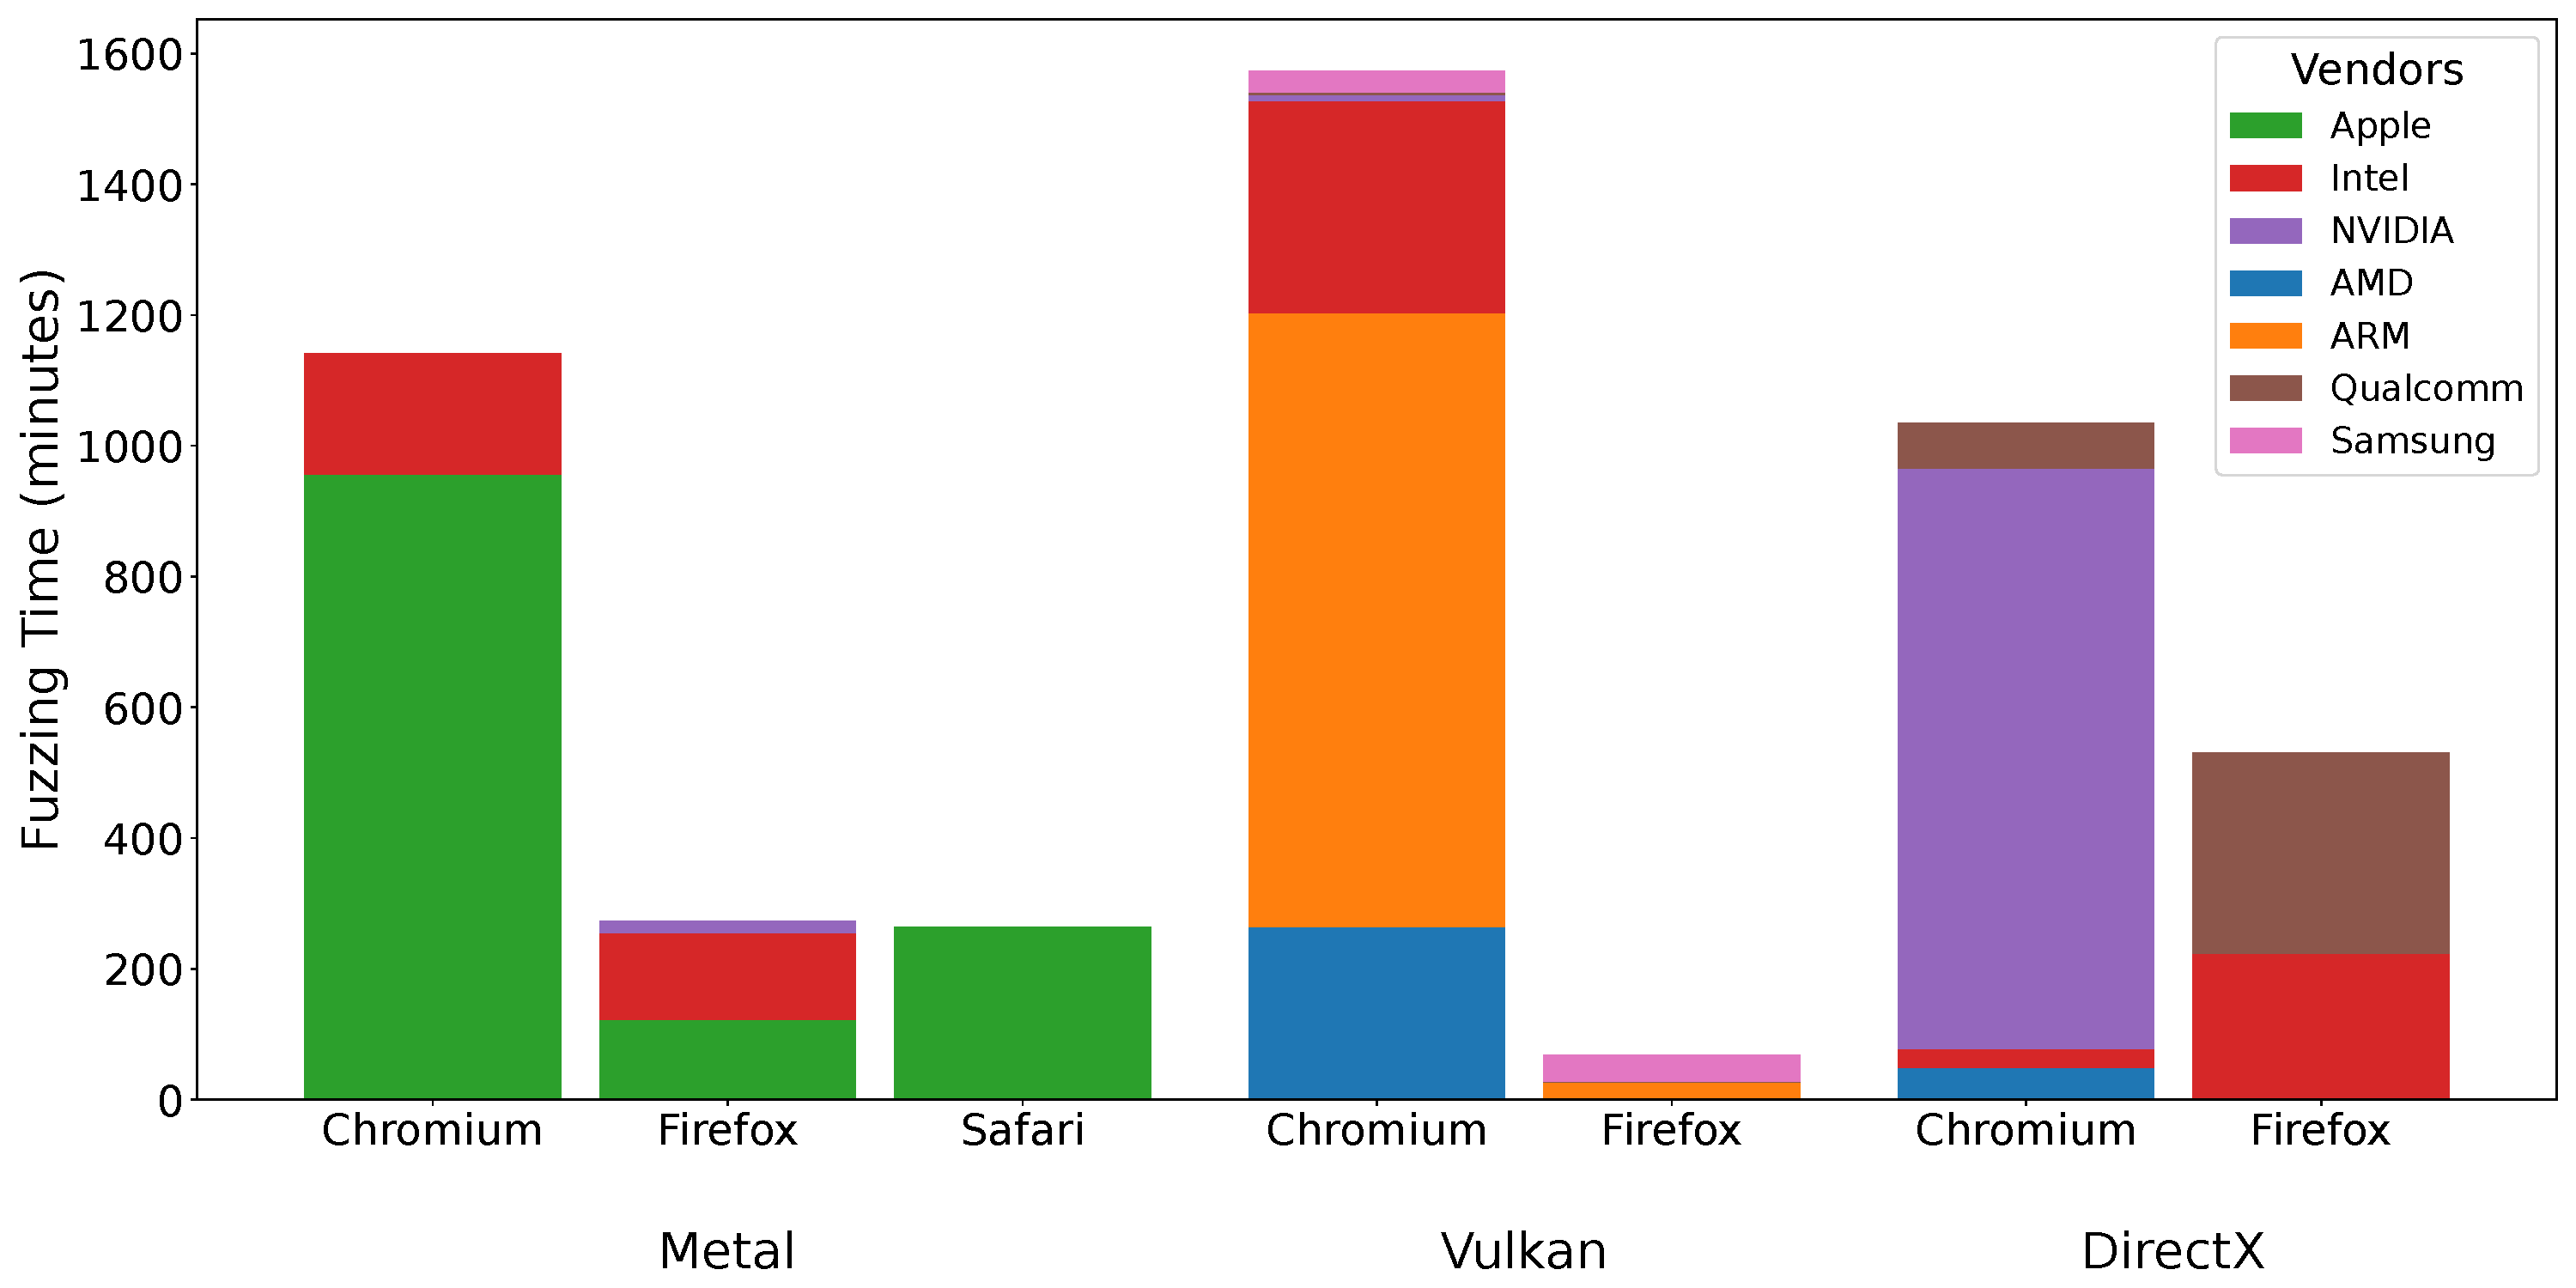
\includegraphics[width=\columnwidth]{images/tracking.pdf}
    \caption{\wgslmemsmith fuzzing time broken down by compilation stack.}
    \Description[Fuzzing Time]{Broken down by backend and vendor. On Metal, we tested on Chromium, Firefox, and Safari, mostly on Apple GPUs but also on Intel, AMD, and NVIDIA. On Vulkan, we tested on Chromium and Firefox, across many vendors: AMD, Arm, Intel, Samsung, Qualcomm, NVIDIA. On DirectX, we tested on Chromium and Firefox as well, on many of the same vendors.}
    \label{fig:fuzzing-time}
\end{figure}

\subsection{Evaluation \label{sec:assess-td-eval}}

We developed a website which runs shaders generated by \wgslmemsmith through WebGPU's JavaScript API and utilized it to test 21 unique compilation stacks. Overall, \wgslmemsmith ran for over 81 hours and tens of millions of unique thread executions, with \myfig\ref{fig:fuzzing-time} breaking down the testing time on different compilation stacks. While we ran fuzzing on both the Chrome and Edge web browsers, we combine these results in our report as they are both built on the Chromium open-source browser and rely on the same underlying WebGPU implementation.

\subsubsection{Testing for Vulnerabilities\label{sec:assess-td-eval-vuln}}
Our fuzzing campaign led to a negative result--data races did not cause memory isolation vulnerabilities due to bounds-checks being optimized away. While this is not a formal proof of the absence of such optimizations, it shows that exploiting the WGSL specification vulnerability is at the least very difficult, and compilers just might not implement the types of optimizations that could cause it today. Despite the lack of observable security concerns, the specification vulnerability is still a ticking time bomb for WGSL's memory safety, and there is no guarantee that compilers won't implement it in the future.

While testing a pre-release version of Firefox on a laptop running Windows with a Qualcomm GPU, we observed non-zero values when reading from out-of-bounds indexes in workgroup memory. Our investigation showed that the Firefox WGSL compiler was not adding bounds-checks correctly for workgroup and private memory. This vulnerability was confirmed by Mozilla privately and fixed in its implementation of WebGPU~\cite{wgpu-oob}. As WebGPU was not available in Firefox's release browser at the time of our discovery, this vulnerability luckily did not impact most users.

%Our results also show that WGSL compilers can introduce data races due to clamping. We observed that WGSL compilers clamp out-of-bounds writes to instead modify the last index in a buffer, and if this index is concurrently read or write a data race occurs. The undefined semantics of data races in native languages break the ability to reason about the resulting program, leading to potentially unexpected behaviors and increasing security risk.

%\paragraph{Testing \smsg Property 2 Adoption Feasibility} On the majority of the compilation stacks we tested (19/29), we did not observe cases where data races affected unrelated variables. However, tests on the remaining compilation stacks did observe cases where adding unrelated statements and potential data races caused the values of safe memory locations to change. The exact configurations of these stacks will be provided in supplemental material upon publishing. The violations varied across components (browser, lower-level framework, GPU), without any specific component being obviously responsible.

%we did not notice any common component of the configurations (GPU, intermediate framework, or browser) for which violations were observed. %These stacks were: a Samsung GPU running under the Vulkan framework, a Qualcomm GPU and an NVIDIA GPU running under the DirectX framework, and an Intel GPU running under the Metal framework.

%There is a chance these outcomes are due to compiler bugs, which have been shown to be relatively common in GPUs~\cite{lidbury2015clsmith}, but exploring these bugs further would require a reducer like C-Reduce~\cite{regehr2012creduce} built into the browser. Research on CPUs has hypothesized that compilers do not implement the transformations that lead to data races affecting unrelated accesses, so it would be surprising if this were the case on GPUs. However, to adopt the semantics of \smsg Property 2, GPUs will need to be thoroughly tested and these observations root-caused, which we leave to future work.

%Our results also showe that WGSL compilers can introduce data races due to clamping, specifically on Metal backends running through the Chrome browser. We observed that clamping writes modify the last index in a buffer, and if this index is concurrently read or write a data race occurs. The undefined semantics of data races in the Metal framework break the ability to reason about the resulting program, increasing security risks and motivating the adoption of our weak semantics.

\begin{table}
\centering
\caption{Percentage of shaders showing memory isolation failures on an Apple M3/M2 GPU with bounds-checks disabled.}

\begin{tabular}{l r r r r r r r}
\toprule
& \multicolumn{6}{c}{\textbf{Memory}} \\
\cmidrule(lr){3-7}
& \multicolumn{2}{c}{\textbf{Private}} & \multicolumn{2}{c}{\textbf{Workgroup}} & \multicolumn{2}{c}{\textbf{Device}} \\
\cmidrule(lr){2-3} \cmidrule(lr){4-5} \cmidrule(lr){6-7}
\textbf{Pattern} & \textbf{M3} & \textbf{M2} & \textbf{M3} & \textbf{M2} & \textbf{M3} & \textbf{M2} \\
\cmidrule(lr){1-1}
\textbf{Basic:} & $4.5\%$ & $0.9\%$ & $4.5\%$ & $3.3\%$ & $37.3\%$ & $18.6\%$ \\
\textbf{UndefArith:} & $5.4\%$ & $4.3\%$ & $3.0\%$ & $3.7\%$ & $3.6\%$ & $3.1\%$ \\
\textbf{ControlFlow:} & $8.2\%$ & $6.1\%$ & $1.0\%$ & $0.0\%$ & $37.8\%$ & $20.4\%$ \\
\bottomrule
\end{tabular}
\label{tab:mut-testing}
\end{table}

\subsubsection{Mutation Testing} To provide more confidence in our testing, we perform mutation testing~\cite{mutation-testing} where we analyze the ability of \wgslmemsmith to observe memory isolation failures in the absence of bounds-checks. These could be missing due to compiler bugs, e.g., the Firefox vulnerability described in \mysec\ref{sec:assess-td-eval-vuln}, or unsound optimizations in the presence of data races, e.g., the examples in \myfig\ref{fig:oob-example} and \mylisting\ref{list:c-code}. We utilize a flag in the Chromium browser to disable bounds-checks on two GPUs, an Apple M2 and M3. As shown in \mysec\ref{sec:assess-bu-eval}, when programs written in Apple's native Metal shading language with memory safety violations were run, these GPUs revealed memory isolation failures. Therefore, we would expect our fuzzing to catch these failures with bounds-checks disabled. For each mutation testing trial, \wgslmemsmith is configured to produce one of the three types of patterns from \myfig\ref{fig:patterns}, i.e., \textbf{Basic}, \textbf{UndefArith}, and \textbf{ControlFlow}:

Each pattern type is then combined with each memory region, private, workgroup, or device, and shaders are generated and run for five minutes on each GPU. The results in \mytab\ref{tab:mut-testing} show the percentage of generated shaders that led to memory isolation failures on each GPU. Every combination except control flow dependence and workgroup memory on the M2 showed isolation failures, validating that \wgslmemsmith can observe failures (in most cases) due to data races if bounds-checks are removed.

%These results also show that in these compilation stacks provably dead code conditionals are not being removed, as otherwise vulnerabilities would not be observed using the control flow pattern.

%While testing, we also observed that a combination of private memory and undefined arithmetic patterns led to data races violating \smsg Property 2 on the M2, and that this behavior disappeared when bounds checks were restored. This result highlights why Property 2 only applies to otherwise well-defined programs; undefined behavior anywhere else in a program may cause unexpected results.

\subsubsection{Register Pressure}
We analyze whether the shaders generated by \wgslmemsmith are causing register pressure on various GPUs, as we discussed in \mysec\ref{sec:extended-example} how this could lead to dangerous optimizations. We utilize a Vulkan extension, \textit{pipeline executable properties}, which allow developers to analyze statistics about shaders. We first randomly generate a shader with \wgslmemsmith using the same limits as in our fuzzing campaign. Next, we use the Tint WGSL compiler to generate a SPIR-V shader, set up a short program that accepts the shader as input, compiles it, and returns the shader statistics, which we report for three GPUs below. %Our results show definitively that \wgslmemsmith is causing register pressure on many of the GPUs we target.

\paragraph{Intel Arc A770 Graphics} There are three relevant statistics reported by Vulkan on this GPU: max live registers, spill count, and fill count. To the best of our knowledge, spill count and fill count measure the number of register spills and re-load instructions which the compiler adds to the shader. For the shader we test, the max live registers is reported as 331, the spill count as 683, and the fill count as 1952, showing that register pressure is indeed occurring.

\paragraph{AMD Radeon RX 7900 XT} Several relevant statistics are reported by Vulkan on this GPU: compiler VGPR/SGPRs, used VGPR/SGPRs, and scratch memory usage. VGPR (SGPR respectively) stands for vector (scalar) general purpose registers, which are used when each thread in a SIMD unit operate on different (the same) data. For the shader we test, the compiler reports 256 available VGPRs and 106 available SGPRs, and uses 256 VGPRs as 37 SGPRs. Our current implementation of \wgslmemsmith focuses on maximizing registers per thread which explains why SGPRs are not maximized---future versions of \wgslmemsmith might be able to address this deficiency. We observe that the final statistic, scratch memory usage is 0 when VGPRs are not maximized, and increases when they are (for our test shader, the value is 496 bytes). Therefore, we can infer that our test shader is causing register spilling on this GPU.

\paragraph{NVIDIA GeForce RTX 4070} The only statistic reported by Vulkan on this GPU is used register count---for our test shader, this value is reported as 255. This number matches the reported maximum number of registers per thread on NVIDIA's Ada GPU architectures~\cite{nvidia2024cudaada}, meaning that the shader is at least utilizing all available registers.

\section{The \saferace Memory Safety Guarantee \label{sec:saferace}}

Our threat assessments, along with vulnerabilities found in prior work~\cite{cuda-leaks, stealing-webpages, leftover-locals, guo2024usenix}, show that GPUs memory isolation vulnerabilities continue to be a serious concern. And although the specification vulnerability in WGSL does not currently seem exploitable, the optimizations which would make it so are valid and could legitimately be implemented at any time by GPU compilers. Therefore, we introduce the \saferace Memory Safety Guarantee (\smsg), which fixes the WGSL \drsv by ensuring that bounds-checks are robust in the presence of data races.

Consider a WGSL program $P_u$, which may contain unsafe behaviors. When $P_u$ is compiled to lower-level languages, it is transformed into $P_s$ by inserting checks to guard against unsafe behavior, e.g., \textcolor{red}{\texttt{min}} in \myfig\ref{fig:oob-example}. However, as described in \mysec\ref{sec:spec-vuln} and \mysec\ref{sec:assess-td-eval-vuln}, WGSL compilers include no special protections against data races and may in fact introduce data races. Compiler transformations in the lower-level language can transform $P_s$ into a new program $P_s'$. Under current specifications, if either $P_u$ or $P_s$ contain data races, $P_s'$ may contain memory safety violations, e.g., \myfig\ref{fig:oob-example} with the \textcolor{red}{\texttt{min}} check removed. To address this, \smsg consists of two properties which when combined ensure that $P_u$ is safe from the \drsv. This in turn ensures that in the absence of other undefined behavior (or compiler bugs), valid transformations from $P_s$ to $P_s'$ are also safe.

\begin{itemize}
    \item \textbf{Property 1: Race-Free Indexing Slices:} Program slices which contribute to memory indexing must be race-free.
    \item \textbf{Property 2: Data Race Non-Interference:} In the absence of other undefined behavior, data races cannot affect the behaviors of race-free slices of programs.
\end{itemize}

We now formally describe a logic for constructing program slices which contribute to memory indexing and walk through a couple examples of how to apply this logic.

\begin{table}
\small
\caption{\saferace Memory Logic}
\centering
\begin{tabularx}{.65\columnwidth}{ l l l }
\toprule
\textbf{Program} & $P$ & The program under analysis \\
%\multicolumn{3}{c}{\textbf{Program} $P$} \\
\midrule
\multirow{2}{*}{\textbf{Memory Scope}}
 & \multirow{2}{*}{$R^{p|w|d}_i$} & Private/workgroup/device \\
 & & memory region \\
\midrule
\multirow{2}{*}{\textbf{Memory Type}}
 & $R^{\{p|w|d\}na}_i$ & Non-atomic memory \\
 & $R^{\{w|d\}a}_i$ & Atomic memory \\
\midrule
\multirow{6}{*}{\textbf{Memory Accesses}}
& $A^{\{r|w|i\}}_x$ & Read/write/initialization access \\
& $A_x.R_i$ & Memory region accessed \\
& $A_x.I$ & Index dependencies \\
& $A_x.C$ & Control dependencies \\
& $A_x.D$ & Data dependencies \\
& $A_x.S$ & Slice: \footnotesize $(A_x.I \cup A_x.C \cup A_x.D)+$ \\
\midrule
\multicolumn{3}{c}{\textbf{Applying \smsg}} \\
\textbf{Property 1} & \multicolumn{2}{l}{\footnotesize $\forall A_y \in (A_x.I \cup A_x.C)$: \texttt{mkAtomic}($A_y.R_i$) $\wedge$}  \\
(\footnotesize \textsc{RaceFreeSlice}) & \multicolumn{2}{l}{\footnotesize $\forall A_z \in A_y.S$: \texttt{mkAtomic}($A_z.R_i$)} \\
\cmidrule(lr){2-3}
\textbf{Property 2} & \multicolumn{2}{l}{\footnotesize $\forall A_x, A_y \in P.A: A_x \neq A_y \wedge A_y \notin A_x.S \implies $} \\
(\footnotesize \textsc{RaceInterference}) & \multicolumn{2}{l}{\footnotesize \texttt{bhvrs}$(A_x) \mid P.A$ $\equiv$ \texttt{bhvrs}$(A_x) \mid P.A\setminus A_y$} \\
\bottomrule
\end{tabularx}

\label{tab:sig-reasoning}
\end{table}

\subsection{A Memory Logic for WGSL \label{sec:sr-reasoning}}

\mytablong\ref{tab:sig-reasoning} shows the constructs used to reason about memory safety in WGSL and the languages it targets. WGSL provides a more restricted programming model than other low-level languages, e.g., C++, which we take advantage of to construct our memory logic. A program $P$ operates on data which is either constant, e.g., literals and program constants, or in disjoint memory regions $R$\footnote{Writable memory bound to a shader cannot alias in WebGPU~\cite[\mysec 14.1]{webgpu}.}. A memory region's name is denoted using a subscript, e.g., $R_i$ is the memory region referred to by name $i$. Memory regions can either be private variables/arrays ($R^p_i$), or shared workgroup/device memory ($R^w_i/R^d_i$). Shared memory regions can either be non-atomic ($R^{\{w|d\}na}_i$) or atomic ($R^{\{w|d\}a}_i$).

A memory region is a fixed-size set of 8-bit memory locations. The type of all memory locations in a region is the same, with casting between atomic and non-atomic references to the region prohibited. %If a memory region contains memory locations with a type of size $s$ bytes, indexing that region accesses a set of $s$ contiguous memory locations.
The set of static memory accesses within a program, i.e., those present in the source code, is represented by $A$. Read and write accesses are represented by $A^r/A^w$, respectively. Declarations of input buffers to a program are represented as a special \textit{initialization} access type $A^i$. Each memory access is given a unique id $x$ which we denote using a subscript on $A$. Each access $A_x$ has several fields, namely: $A_x.R_i$ denotes the memory region accessed; $A_x.I$ are the index dependencies, i.e., the set of accesses which potentially contribute to the calculation of the index into $A_x$; $A_x.C$ are the accesses on which $A_x$ is control-dependent; and $A_x.D$ are the accesses on which $A_x$ is potentially data-dependent, which for a read access $A^r_x$ are the set of accesses it may read from, and for a write access $A^w_x$ are the set of accesses which determine the value written.

Because our approach is based on static analysis, we say that an access $A_x$ is \textit{potentially} dependent on an access $A_y$ if there exists an assignment of values, e.g., due to data races or conflicting atomic accesses, to other accesses in the program that causes $A_x$ to be dependent on $A_y$. Intuitively, this means conditionals based on shared memory read accesses may resolve to any branch and assuming a write access with an index dependency on a shared memory read access may write to any location in a memory region $R_i$. This ensures that any calculation of $A_x$'s dependencies is sound, but potentially an over-approximation. %In addition, clamping inserted by WGSL compilers may create potentially dependent relationships between accesses that do not exist in the original source code, which must be taken into account when constructing dependencies.

The transitive closure of the union of $A_x.I$, $A_x.C$, and $A_x.D$ is called the access \textit{slice}, or $A_x.S$. A slice represents all memory accesses which may affect $A_x$, including its reachability, the memory locations it accesses, the value stored if $A_x \in A^w$, and the value it returns if $A_x \in A^r$. $A_x.S$, along with its constituent sets, can be obtained via static program slicing based on a data-flow and control-flow analysis~\cite{weiser1984slicing}.

The definition of an access now allows us to precisely define how to reason about programs with \smsg. Property 1 can be enforced by a compiler in a safe high-level language via the rule \textsc{RaceFreeSlice} in \mytab\ref{tab:sig-reasoning}. This rule specifies that given an access $A_x$, for all accesses $A_y$ in $(A_x.I \cup A_x.C)$, if $A_y.R_i$ is a shared memory region it must be made atomic. Additionally, for all accesses $A_z$ in the transitive closure of $A_y.S$, if $A_z.R_i$ is a shared memory region, it also must also be made atomic (note that \texttt{mkAtomic()} is a no-op for private memory regions and that when applying \textsc{RaceFreeSlice} to $A_x$, $A_x.D$ is not included because the data dependencies of $A_x$ do not determine the memory locations in $R_i$ $A_x$ accesses). Intuitively, the program slice for each index and control dependency of an access is now race-free as all contributing memory accesses have been made atomic, preventing the optimizations discussed in \mysec\ref{sec:spec-vuln} and \mysec\ref{sec:extended-example}.

Property 2, which must be adopted by the memory-safe language \textit{and} the languages in its compilation stack, specifies that if a memory access $A_y$ is not in $A_x.S$, it cannot affect the result of $A_x$ even if it participates in a data race. Therefore, when running a program $P$, the possible behaviors of $A_x$, i.e., \texttt{bhvrs}($A_x$), with $A_y$ included in $P$ must be equivalent to the possible behaviors of $A_x$ when running $P$ with $A_y$ removed.

\lstdefinelanguage{wgsl}{
    mathescape,
    literate={->}{$\rightarrow$}{2},
    keywords=[1]{@group, @binding, var, fn, @compute, @workgroup_size, @builtin}, % WGSL-specific keywords
    keywords=[2]{device, workgroup, array, vec3, i32}, % WGSL types and storage classes
    sensitive=true, % WGSL is case-sensitive
    morecomment=[l]{//}, % line comments
    morecomment=[s]{/*}{*/}, % block comments
    morestring=[b]", % strings
    keywordstyle=[1]\color{blue}\bfseries, % styling for keywords
    keywordstyle=[2]\color{teal}, % styling for types and storage classes
    commentstyle=\color{gray}\itshape, % styling for comments
    stringstyle=\color{orange}, % styling for strings
    numbers=left, % line numbers on the left
    numberstyle=\tiny\color{gray}, % line number style
    stepnumber=1, % show every line number
    numbersep=5pt, % distance between line numbers and code
    showstringspaces=false, % do not show spaces in strings
    basicstyle=\ttfamily\small,
    breaklines=true, % allow line breaks
    tabsize=4, % tab width
    captionpos=b, % positioning of captions
    escapebegin=\color{gray},
}

\begin{figure}[t]
    \centering
    \begin{lstlisting}[language=wgsl, caption={WGSL pseudocode illustrating how to reason using our memory logic.}, label={list:smsg-reasoning}, basicstyle=\small, xleftmargin=10pt, xrightmargin=10pt]
var<device>    a: array<i32, 1>; $A^i_0:  \{R^{dna}_a\}$
var<device>    b: array<i32,10>; $A^i_1: \{R^{dna}_b\}$
fn shader() {
  a[0]=5;       $A^w_2: \{R_a\}$
  var x:i32=3;  $A^w_3: \{R^{pna}_x\}$
  if(a[0]>5)    $A^r_4: \{R_a, D=\{A^w_2\}\}$
    x=100;      $A^w_5: \{R_x, C=\{A^r_4\}\}$
                $A^r_6: \{R_x, D=\{A^w_5, A^w_3\}\}$
  var r=b[x+1]; $A^r_7: \{R_b, I=\{A^r_6\}\}$
}
    \end{lstlisting}
    \Description[Applying SMSG]{Code showing how to apply SMSG reasoning to an example WGSL program. The code is explained below in the larger example paragraph.}
\end{figure}

\subsection{Applying \smsg}

First, we show how \smsg can be applied in the simple examples in \myfig\ref{fig:oob-example}, and then move on to a more complex example which includes control flow and multiple types of dependencies.

\paragraph{Simple Example}
In both programs in \myfig\ref{fig:oob-example}, there are two memory regions which we assume are device-scoped---\texttt{i} ($R^{dna}_i$) and \texttt{m} ($R^{dna}_m$)---and one private memory region---\texttt{x} ($R^p_x$). In \myfig\ref{fig:oob-example-a}, the access to \texttt{m} is index-dependent on the access to \texttt{i[0]}, so applying \textsc{RaceFreeSlice} means compiling $R^{dna}_i$ to $R^{da}_i$, thereby making all accesses to \texttt{i[0]} atomic. Because accesses are now atomic, the compiler cannot assume that \texttt{i[0]}'s value won't change between accesses, and thus, cannot erroneously remove the bounds-check. In \myfig\ref{fig:oob-example-b}, $R^p_x$ is race-free as it is a private memory region, and applying \textsc{RaceInterference} means that the data race on $R^{dna}_i$ cannot affect it.

\paragraph{Larger Example}
\mylistinglong\ref{list:smsg-reasoning} shows an example of how to apply this logic to a program $P_u$. There are six memory regions in $P_u$: $R^{dna}_a$, $R^{wna}_b$, $R^{wna}_c$, $R^{dna}_d$, $R^p_x$, and $R^p_r$. All memory events, including the declaration of buffers on lines 1-4, are represented as memory accesses. Only non-empty base fields are shown, with the type of a memory region omitted after its first reference.

Accesses and their dependencies are shown either above or on the line they reference, so the accesses on lines 12-15 all correspond to the code in line 15. Working backwards from line 15, $A^r_{13}$ is index-dependent on $A^r_{11}$ and $A^r_{12}$. $A^r_{11}$ is potentially data-dependent on $A^w_6$ and $A^w_8$, while $A^w_8$ is control-dependent on $A^r_7$. Meanwhile, $A^r_{12}$ is data-dependent on $A^w_{10}$, which in turn is data-dependent on $A^r_9$. At this point, every memory region besides $R_d$ and $R_r$ in $P_u$ is contained in accesses in $A^r_{13}.S$.

Assuming the absence of data races, which a compiler for an unsafe language can do since all memory regions are non-atomic, all bounds-checks in this example could be provably removed as the index on line 15 evaluates to 5. However, data races may cause these values to change in ways that break memory safety. For example, a race on \texttt{c[0]} or \texttt{b[0]} could cause their values to increase even after the compiler has removed the bounds check, as \myfig\ref{fig:oob-example} and \mylisting\ref{list:c-code} showed. Similarly, a race on \texttt{a[0]} could cause the code in the conditional to execute despite the compiler optimizing based on the determination that it is dead code\footnote{Since it is dead code, a compiler might decide to eliminate it, in which case $R_a$ does not need to be made atomic. However, GPUs execute in a single-program multiple-data manner, so dead code in one thread may not be dead in another and a compiler may decide to leave it in place.}.

When compiling from $P_u \rightarrow P_s$, applying Property 1 via \textsc{RaceFreeSlice} means compiling memory regions as follows: $R^{dna}_a \rightarrow R^{da}_a$, $R^{wna}_b \rightarrow R^{wa}_b$, and $R^{wna}_c \rightarrow R^{wa}_c$. Legal transformations $P_s \rightarrow P_s'$ cannot assume the value of atomic memory locations, prohibiting optimizations that both remove the bounds check and rematerialize from the shared memory regions in accesses in $A^r_{13}.S$. The other memory region in accesses in $A^r_{13}.S$, $R^p_x$, is not made to shared memory, \textsc{RaceInterference} ensures that its value cannot be affected by data races elsewhere in the program.

\subsection{\smsg Soundness}

We now argue that the rules for applying \smsg ensure that data races cannot lead to memory safety violations. Consider a program $P_u$ which contains a memory access $A_x$ that may attempt to read out-of-bounds memory. In an initial compilation from $P_u \rightarrow P_s$, e.g., WGSL to a lower-level language, $A_x$ is compiled to $A'_x$, which is guaranteed to not read out-of-bounds due to checks added by the compiler. Now, assume a valid transformation $T$ in the lower-level language compiles $A'_x \xrightarrow{T} A''_x$, and that $A''_x$ no longer contains bounds-checks and leads to a memory safety violation.

If Property 1 is applied correctly, there are no data races in $B$, the set of memory accesses in $A'_x.I$ and $A'_x.D$ and in their slices. Therefore, any analysis the compiler performs to remove the bounds-check in $A''_x$ while considering the values of memory accesses in $B$ is safe. The only other source of data races in $P_s$ are accesses not in $B$, which cannot affect the behaviors of accesses in $B$ according to Property 2. As $B$ is exactly the set of accesses that contribute to the calculation of $A'_x$'s (and therefore $A''_x$'s) index, $A'_x$ and $A''_x$ are safe. This means that if $T$ is a valid transformation, it must have introduced the memory safety violation due to behaviors other than data races, validating our claim that $P_s$ is safe in the presence of data races.

\paragraph{Complete Memory Safety in WebGPU}

Enforcing \smsg ensures that data races no longer lead to globally undefined behavior or memory safety violations due to out-of-bounds accesses. However, to provide complete memory safety, WebGPU needs to guarantee that no possible WGSL program can lead to undefined behavior in its lower-level language targets.
%WGSL needs to guarantee that no valid programs can lead to undefined behavior.
The current WGSL specification avoids undefined behavior by classifying its common sources, including data races, as dynamic errors, but as we have shown this is not necessarily sufficient. Therefore, we analyze the other sources of dynamic errors mentioned in the specification, which are: aliased writable memory bound to a shader~\cite[\mysec 7.3]{wgslspec}, mismatched memory layouts~\cite[\mysec 13.4]{wgslspec}, unbounded loops~\cite[\mysec 9.4.3]{wgslspec}, and an erroneous graphics-specific vertex value~\cite[\mysec 12.3]{wgslspec}.

Non-aliasing of memory is enforced by the WebGPU host API~\cite[\mysec 14.1]{webgpu}, and while mismatched memory layouts between the host/shaders can affect correctness of programs, the values in memory do not change the analysis used to apply \smsg. We do not consider graphics pipelines, leaving unbounded loops as the last source of dynamic errors. Unlike in languages like C++, where unbounded loops with side effects are useful for many tasks, GPU languages are generally not designed for long-running programs. In fact, most GPU languages currently lack a well-specified forward progress model~\cite{sorensen2021progress}, so even unbounded loops with side effects often lead to crashes or other issues. The lack of support for unbounded loops has impacts on memory safety, and open-source WGSL compilers insert some code in response to the fact that the Metal compiler might optimize away bounds-checks due to considering infinite loops without side effects undefined behavior~\cite{wgpuIssue4972}. While so far this approach seems be successful, the lack of specificity around the behavior of unbounded loops means that we currently only apply \smsg guarantees to source programs that are free of behaviors like unbounded loops.

\subsection{Other Memory Safety Approaches}

There are several other approaches which could be used to avoid the removal of bounds-checks and help maintain memory safety in WGSL. The first, and simplest, is to simply enforce that all memory accesses are made atomic when compiling from WGSL to lower-level GPU languages, which would remove data races from all programs. However, even though the \texttt{relaxed} memory order semantics for atomics which we use are less costly than more heavyweight memory orders like \texttt{acquire}/\texttt{release} and sequentially consistent, our results in \mysec\ref{sec:smsg-prop-1-eval} show that in cases where some accesses must be made relaxed atomic operations, there is already a performance decrease. Making every access atomic likely would cause unacceptable performance for many applications.

Another option is LLVM's \texttt{unordered} atomic ordering~\cite[Atomic Memory Ordering Constraints]{LLVM_LangRef} for all accesses, which provides weaker semantics than \texttt{relaxed} but prevents rematerializing loads and is used by LLVM to match Java's memory model. However, the languages which WGSL targets, e.g., SPIR-V, Metal, and HLSL, do not all explicitly support unordered atomics yet. To implement this solution, the changes in GPU compiler implementations and the performance of using unordered atomics would need to be carefully studied and tested. Additionally, \smsg can be integrated with unordered atomics, as Property 1 can translate access dependencies to unordered atomics instead of relaxed atomics, while Property 2 is weaker than unordered atomic guarantees.

A different style of approach is to integrate some form of ``unoptimizable checks'' into WGSL and the languages it targets. For example, LLVM has a concept of \textit{linkage types}~\cite[Linkage Types]{LLVM_LangRef}, including types like \textit{weak} which prevent a compiler from removing unreferenced global variables and functions. If the \texttt{min} function is declared using this attribute, the compiler would therefore not be able to remove it. While this approach is promising, unoptimizable checks would require a large amount of coordination and implementation work across WGSL and the languages it targets. Also, to our knowledge, the guarantees offered by existing unoptimizable checks like linkage types are not formally defined in relation to existing sources of undefined behavior such as data races. On the other hand, \smsg is a novel solution to memory safety in the presence of data races using existing language constructs that are preserved across all target languages, i.e., relaxed atomic accesses.

%\begin{table}
%\footnotesize
%\centering
%\caption{Impact of applying \smsg Property 1 to Rodinia CUDA benchmarks running on an NVIDIA RTX 4070.}
%\begin{tabular}{l r r r }
%\toprule
%\textbf{Benchmark} & \textbf{Affected Regions} & \textbf{\# of Accesses} & \textbf{Perf. Impact} \\
%\midrule
%\textbf{b+tree} & 4 & 25 & 1.91\% \\
%\textbf{bfs} & 2 & 6 & 5.38\% \\
%\textbf{heartwall} & 1 & 3 & 1.43\% \\
%\textbf{myocyte} & 1 & 155 & 40.44\% \\
%\textbf{particlefilter} & 1 & 5 & 1.56\% \\
%\bottomrule
%\end{tabular}
%
%\label{tab:rodinia}
%\end{table}

\section{Implementing \smsg Property 1 \label{sec:smsg-prop-1}}

We implemented Property 1 as a pass in Tint, the WGSL compiler included in the Dawn WebGPU implementation used by Chromium. %We chose Tint over the other open source WGSL compiler, Naga, included in Firefox as part of the Wgpu WebGPU implementation, because at the time of development Tint was a more complete implementation of the WGSL specification and WebGPU was fully available as part of Chromium's releases.
While Tint is not an optimizing compiler, it does include significant infrastructure for performing passes on WGSL programs, e.g., inserting bounds-checks and ensuring arithmetic expressions are well defined. Tint converts WGSL programs into an intermediate representation (IR) in static single-assignment (SSA) form and includes utilities for traversing and modifying the IR.

Our pass consists of two phases: a backwards slicing phase and a forward conversion phase. In the slicing phase, the \textsc{RaceFreeSlice} rule is applied to compute the sets of accesses which contribute to an access $A_x$. In the conversion phase, non-atomic memory regions are converted to atomic regions, and every usage of these regions is updated to atomically load or store to them. Our implementation accounts for nested types, e.g.., arrays and structs, handles control flow, e.g., loops and branches, and performs complete interprocedural analysis. In the process of writing our implementation, we encountered several constructs that either provided opportunities for optimization or exposed limitations in WGSL. We now detail these constructs as they provide interesting avenues for future WGSL development.

\paragraph{Read-Only Regions} All WGSL memory regions have an \textit{access mode}, either \texttt{read}, \texttt{read\_write}, or \texttt{write}. During our calculation of Property 1, if we encountered a read-only region, we did not convert it to atomic, because by definition reads cannot race with each other in the absence of a write. However, in some cases it is possible that even if a region is marked as \texttt{read\_write}, it is only read to during execution of the shader. While not implemented, regions which are only read from, even if marked \texttt{read\_write}, do not need to be accessed atomically.   %We did not implement the necessary analysis to avoid atomic translation of regions that are in practice only read to, but if WGSL compilers were able to run this analysis, they might enable optimization opportunities not being taken advantage of today.

%\paragraph{Structs and Compound Types} In WGSL, it is possible to define structs consisting of types with different fields, and to arbitrarily nest structs and arrays. In some cases, our analysis required converting only one field of a struct or the innermost type of a nested array to an atomic type. In Tint's IR, accesses to inner compound types are converted into a list of access indices to traverse the type, so our analysis had to keep track of this list during backwards slicing in order to determine which field of a struct needed to be converted.

\paragraph{Limitation on Atomic Types} WGSL currently only allows two atomic types: unsigned and signed 32-bit values. This has implications for both the completeness and performance of our implementation of Property 1. For example, one element of a \texttt{vec2} may be included in the index dependency of an access, but since a \texttt{vec2} cannot be made atomic, we cannot convert it and ensure it won't participate in a data race. Similarly, if a floating point value is part of the control dependency of an access, the region the floating point is loaded from can't be converted. Therefore, it is currently not possible to implement Property 1 completely in WGSL. When our implementation encounters a data type that cannot be accessed atomically in WGSL, it is flagged so that users of the compiler pass can be made aware of the issue. For example, safety critical applications may decide to discard flagged shaders and perform the computation on the CPU instead. In the future, WGSL could add support for atomic floats and other data types, following the example set by C++, which implements an atomic type template which can be applied as long as certain \textit{named requirements} are satisfied~\cite{cppreferenceAtomic}.

The limitations on atomic types also impact the performance of shaders translated by our pass. In WGSL, atomic types are not \textit{constructible}, i.e., able to be loaded/stored directly, passed into functions, or created outside of the declarations of buffer types. If a struct or sized array which contains a type converted by our pass is loaded into a private variable, a function loads each field of the struct or loops over the array and loads each element. It is not possible to directly load a runtime-sized array, creating an upper bound on the number of accesses which must be made atomic. WGSL's ability to support atomic types is dependent on their implementation in native GPU languages. These languages are slowly adding support for more atomic types, so future enhancements to WGSL can increase the coverage of \smsg Property 1. For full completeness, however, it may be required to limit the types which can contribute to memory accesses.

%\paragraph{Control Flow} Our implementation handles all types of control flow statements supported by WGSL, as well as analysis across functions. Due to the way in which loops are structured in Tint's IR, our analysis is overly conservative and may unnecessarily convert some types, providing an opportunity for future optimization.

%\paragraph{Interprocedural Analysis} Every WGSL program is contained in a single file, with a single entrypoint function that is dispatched on the GPU by the host. This allows us to perform a complete interprocedural analysis on the program, traversing function calls to search for contributing shared memory accesses. Shared memory regions may either be passed into functions as pointer arguments, or directly accessed from within the function. Our analysis also requires mapping function parameters to the arguments which they are called with, as the return value of a function may have data dependencies on shared memory regions the arguments were loaded from.

\paragraph{Targeting Different Backends}
As described in \mysec\ref{sec:ub-sources}, both DirectX and Vulkan provide guarantees that operations on device memory will not execute out-of-bounds, while Metal does not. It may seem then that we do not need to apply \smsg Property 1 to device memory accesses in DirectX and Vulkan. However, these guarantees are more analogous to runtime protections in operating systems, rather than features of the languages themselves. This is because data races in both HLSL and SPIR-V programs are undefined, meaning that memory safety violations could potentially occur in racy programs. In some sense, these could also be considered specification vulnerabilities of DirectX and Vulkan, motivating future work on the development of these frameworks. For our purposes, this means that we apply \smsg Property 1 to all memory operations on all backends.

\begin{table}
\footnotesize
\centering
\caption{Impact of applying \smsg Property 1 to WebGPU benchmarks running on an Apple M3.}
\begin{tabular}{l r r r r r}
\toprule
\textbf{Benchmark} & \textbf{Shaders} & \textbf{Impacted} & \textbf{Impacted} & \textbf{Pass Timing} & \textbf{Runtime}\\
& & \textbf{Shaders} & \textbf{Accesses} & \textbf{(ms)} & \textbf{Overhead} \\
\midrule
\textbf{WebLLM DeepSeek Qwen 7B~\cite{ruan2024webllmhighperformanceinbrowserllm}} & 73 & 4 & 24 & 62.47 & 0.0\% \\
\textbf{WebLLM Llama 3.2 1B~\cite{ruan2024webllmhighperformanceinbrowserllm}} & 63 & 1 & 24 & 53.78 & 0.0\% \\
\textbf{ONNX Runtime (Whisper)~\cite{whisperLargeV3TurboWebGPU}} & 60 & 0 & 0 & 8.67 & 0.0\% \\
\textbf{ONNX Runtime (Phi-3)~\cite{XenovaPhi3WebGPU}} & 19 & 0 & 0 & 3.77 & 0.0\% \\
\textbf{MediaPipe Gemma2 2B~\cite{mediapipeStudioLLM}} & 72 & 0 & 0 & 5.17 & 0.0\% \\
\textbf{FFT Ocean Demo~\cite{FFTOceanDemo}} & 9 & 0 & 0 & 0.11 & 0.0\% \\
\textbf{Game Of Life~\cite{WebGPUSamples}} & 1 & 0 & 0 & 0.08 & 0.0\% \\
\textbf{Compute Boids~\cite{WebGPUSamples}} & 1 & 0 & 0 & 0.03 & 0.0\% \\
\textbf{Bitonic Sort~\cite{WebGPUSamples}} & 3 & 1 & 10 & 0.34 & 9.8\% \\
\textbf{MSM~\cite{DereiKohWebGPU_MSM_BLS12_2023}} & 4 & 3 & 7 & 23.43 & 3.0\% \\
\bottomrule
\end{tabular}

\label{tab:webgpu-benchmarks}
\end{table}


\subsection{Evaluation \label{sec:smsg-prop-1-eval}}

While the goal of \smsg is to prevent malicious actors from exploiting memory safety violations in WGSL programs, its guarantees apply to all WGSL programs. This means that even in programs that are not malicious, the \smsg pass analyzes memory accesses and translates dependencies into atomic operations. Therefore, we conducted a study to evaluate the cost of \smsg Property 1 in terms of both compilation time and GPU performance.

\subsubsection{Benchmarks}

Our implementation of Property 1 in Tint allows us to build a custom version of Chromium on an Apple M3 and run our analysis on a set of WebGPU applications, detailed in \mytab\ref{tab:webgpu-benchmarks}. As WebGPU is still in active development and is not yet fully available on all web browsers, this set of applications consists mostly of demonstrations. We believe these applications provide a good benchmark of how WebGPU can be utilized by browser applications.

The first five benchmarks in \mytab\ref{tab:webgpu-benchmarks} are AI applications. \textbf{WebLLM DeepSeek Qwen 7B} and \textbf{WebLLM Llama 3.2 1B} utilize WebLLM~\cite{ruan2024webllmhighperformanceinbrowserllm} to run LLM inference. Under the hood, WebLLM relies on Apache TVM~\cite{apache_tvm}, specifically TVM's Web runtime, and supports many models. We chose two models for our benchmark: the Llama-3.2-1B-Instruct generative model, and the DeepSeek-R1-Distill-Qwen-7B reasoning model. %These are both state-of-the-art models, exemplify the main types of LLM inference being actively researched today, and are small enough to fit on a typical consumer GPU.
\textbf{ONNX Runtime (Phi-3)} and \textbf{ONNX Runtime (Whisper)} use ONNX Runtime Web~\cite{onnxruntime_webgpu_tutorial} through transformers.js~\cite{transformersjsDocs}, which allows machine learning models to be deployed and run in browsers using WebGPU. The \textbf{Phi-3} benchmark runs inference using the Phi-3-mini-4k-instruct model, while the \textbf{Whisper} benchmark runs speech recognition with OpenAI's Whisper Large V3 Turbo. Finally, \textbf{MediaPipe Gemma2 2B} uses Google's MediaPipe suite to run LLM inference with the Gemma2 2B model.

The other benchmarks consist of demonstrations of WebGPU's compute abilities. Three, \textbf{Bitonic Sort}, \textbf{Game of Life}, and \textbf{Compute Boids}, are part of the WebGPU Samples maintained by the official WebGPU working group~\cite{WebGPUSamples}, \textbf{FFT Ocean Demo} shows how to use compute shaders to render complex ocean waves as part of the Babylon.js library for 3D web graphics~\cite{FFTOceanDemo}, and \textbf{MSM} is a WebGPU implementation of multi-scalar multiplication submitted to the 2023 ZPrize competition~\cite{ZPrize2025}. % which won a special mention for the best WebGPU implementation.
This last benchmark relies on sparse-matrix multiplication techniques, an area where complex index dependencies may be more common than in dense computations.

\subsubsection{Compilation Cost}

Unlike a language like CUDA which is often precompiled to GPU assembly code, WGSL shaders are translated to native GPU languages and vendor-specific machine code at runtime. To mitigate the cost of runtime compilation, WebGPU implementations and native GPU frameworks utilize layered and non-standardized compilation processes, often involving asynchronous operations, just-in-time (JIT) compilation, and caching components. This complex structure makes it difficult to measure the timing of the full compilation pipeline. Therefore, in \mytab\ref{tab:webgpu-benchmarks}, rather than reporting the time taken by our pass as a percentage overhead of the full compilation process, we instead simply report the raw time (in the \textbf{Pass Timing} column) it takes to run our pass on the shaders in each benchmark. %These times also provide a baseline which can be improved as our pass is optimized.}

Compared against only the time taken to run the existing passes in the \texttt{tint} compiler, the addition of our pass adds a large overhead (up to 9x for the slowest-compiling shader in the \textbf{MSM} benchmark). However, these pre-existing passes are generally much simpler, e.g., doing a sequential scan of a shader and adding bounds-checks to memory accesses, while our pass requires relatively complex dependency analysis and program traversal. The timing of passes in the \texttt{tint} compiler also does not include the time it takes to parse WGSL programs into an IR and write them out to native GPU programs, nor the time taken by native language compilers to generate machine code, meaning that the time taken to run all passes is a small part of the overall compilation and runtime process. For example, on the \textbf{WebLLM DeepSeek Qwen 7B} benchmark, the one-time cost of our pass summed across all shaders was only 62.47 ms, while each shader ran dozens to hundreds of times for a total of several seconds during a \textit{single} inference response, with typical LLM interactions usually consisting of many inferences.


%The fact that WGSL code is single-source and typically consists of relatively short programs (10s-100s of lines of code) also reduce compilation costs.

%We measured the time it took to run our pass and total compilation using the \texttt{std::chrono} library when compiling from WGSL to native GPU languages.

%Overall, the compilation cost of running the \smsg Property 1 pass was significant, \update{with the \textbf{MSM} benchmark showing the maximum compilation cost, up to 90\% of the total compilation time}. As our implementation of the pass is naive and unoptimized, we believe that we could reduce these costs with more engineering effort. Even so, compilation costs tend to be a tiny fraction of WebGPU application performance, with average compilation times for shaders ranging from 0.5-2 ms. For example, on the \textbf{WebLLM DeepSeek Qwen 7B} benchmark, the compilation time summed across all shaders was only 179 ms, while each shader ran dozens to hundreds of times for a total of several seconds during a typical inference response, \update{and the \textbf{MSM} shaders all compiled in under 25 ms even with our pass enabled.}

\subsubsection{GPU Performance Cost}

Atomic operations constrain compiler optimizations, and thus, can negatively impact performance~\cite{schweizer2015atomiccost, burtchell2024characterizing}. Therefore, it is likely that any atomic operations added to satisfy \smsg Property 1 could lead to reduced application performance. However, as shown in \mytab\ref{tab:webgpu-benchmarks} in the \textbf{Runtime Overhead} column, on the majority of the benchmarks we tested \smsg Property 1 did not apply to any shaders. We now discuss the four benchmarks where it did apply.

While the two WebLLM model benchmarks differed in the number of shaders used by the program, they both compile a shader called \texttt{apply\_penalty\_inplace\_kernel} which requires making four memory regions atomic, affecting 24 accesses in the program. However, we have received confirmation from the developers of WebLLM that these shaders are not yet used during LLM inference. Additionally, the accesses that must be made atomic in this shader are floating point accesses, and as mentioned in \mysec\ref{sec:smsg-prop-1} WGSL does not yet allow atomic access to floating point data types. Therefore, if WebLLM starts using this shader, we can no longer guarantee memory safety in this application, at least until WGSL begins to support atomic accesses to more data types.

%However, all the memory regions affected ended up being arrays of floating point values, and as mentioned above it is not currently possible to access floating point values atomically in WGSL. Therefore, we cannot determine the performance impact of \smsg Property 1 on this shader. Complicating the matter further, we have determined that this shader is not actually run during LLM inference for either model (hence the 0\% overhead), so we can't determine this shader's impact on LLM inference runtime. We have reached out to WebLLM to understand how this shader is used.

The \textbf{Bitonic Sort} benchmark does require making one workgroup buffer memory region atomic, affecting 10 accesses in one shader. To complete one full sort, using default parameters, this shader runs 91 times. In order to get precise GPU timing information, we extended Dawn's WebGPU implementation to automatically record GPU timestamps for every compute shader. We ran the full sort three times each with our pass enabled and disabled on an Apple M3 GPU, and calculated the average time across the 91 runs of the shader. On average, each shader run took between .04-.09 ms, for a total of 3.6-8.2 ms. With our pass enabled, average runtime of the shaders increased by 9.8\%, from .064 ms per shader to .071 ms. We performed the same analysis on the \textbf{MSM} benchmark; applying \smsg Property 1 to these shaders required making 7 accesses atomic. The average shader runtime of this benchmark increased from .99 seconds to 1.02 seconds, or 3\%.

To conclude, these results show that only \textasciitilde 2\% of the shaders in our benchmarks are affected by \smsg Property 1. The benchmarks consist of important WebGPU applications in several domains, including LLM inference and general compute algorithms, and are either generated by state-of-the-art tensor compilers, e.g., TVM~\cite{apache_tvm}, or handwritten by expert GPU developers.  Despite this, many of the shaders used by these applications do not include the complex indirect memory accesses that require applying transformations to satisfy \smsg Property 1, validating the efficacy of \smsg. For example, matrix multiplication is generally written using simple index calculations taken from combinations of thread identifiers and constants, and none of the matrix multiplications in our LLM benchmarks require any transformation. On the other hand, it is possible that some applications, e.g., bitonic sort, will experience reduced performance due to the safety requirements of \smsg Property 1. We also show that in this set of benchmarks, data types which cannot be accessed atomically in WGSL are generally not used in index dependence calculations, with the only exception being the WebLLM shader which may be utilized in the future. All browser-based languages must make tradeoffs between performance and safety, and we believe our results provide evidence that the performance overhead of adopting \smsg Property 1 is within acceptable limits.

\section{Testing \smsg Property 2 \label{sec:smsg-prop-2}}

While \smsg Property 1 can be implemented by WGSL compilers, Property 2 must be adopted by the languages WGSL targets. This may seem like a thorny problem; many languages, including C++ and GPU languages, leave the behavior of data races undefined to avoid having to reason about constraints like the one required by Property 2. However, previous work on data races has shown how to bound the behavior of data races to provide a local data-race-free (Local DRF) property and proven the soundness of many existing compiler optimizations given this property~\cite{bounding-races}.

The Local DRF property is stronger than \smsg Property 2. It prevents a data race on one memory location $x$ causing an unrelated memory location $y$ to read a value written to $x$, what has been called \textit{bounding data races in space}. It also prevents the effects of data races from leaking across synchronization points, e.g., barriers, called \textit{bounding data races in time}. In particular, bounding data races in time requires preserving load-store ordering, which has been shown to have relatively low cost on CPUs. However, the cost of load-store reordering has not been studied on GPUs, where it is very commonly observed~\cite{levine2023gpuharbor}. Still, prior work showed that preserving load-store ordering is not necessary to bound data races in space, while proving that many existing compiler transformations are compatible with this property~\cite{bounding-races}, and therefore, \smsg Property 2.

To test whether \smsg Property 2 is maintained by current GPU compilers, we augmented the \wgslmemsmith fuzzer using metamorphic fuzzing. When generating shaders, variables and memory locations are split into \textit{safe} and \textit{unsafe} sets. Safe memory locations are read-only or written to by only one thread, while unsafe memory locations may be read or written to by any thread. Safe local variables are only used in combination with safe memory locations, while unsafe variables can be combined in expressions with unsafe memory locations. Intuitively, this process creates race-free slices of programs, as well as slices that may contain races. During fuzzing, we run two shaders, one with only race-free slices and the other with both race-free and racy slices.

The race-free shader is run first and the values in memory at the end of execution are saved. Since this shader contains no data races or sharing of memory between threads, the results are deterministic. The racy shader, which contains the exact statements in the safe shader along with statements that operate on unsafe memory locations and may contain data races, is run next. Then, the values in safe memory locations at the end of the racy shader execution are compared with the values from the race-free shader execution---if the racy shader results differ, the addition of data races may have caused the differences, violating \smsg Property 2.

\subsection{Evaluation}

As we use the same shaders for both the metamorphic fuzzing and testing for \smsg Property 1, our evaluation consists of the same set of compilation stacks and testing time shown in \myfig\ref{fig:fuzzing-time}. On most compilation stacks we tested, we found that data races did not effect race-free slices of programs. This was true for all compilation stacks using Vulkan and DirectX as the WebGPU backend, as well as Metal backends targeting Apple M-series GPUs. On DirectX backends, data races caused unexpected values in unsafe memory locations, i.e., values that could not be explained by any writes to those memory locations, but this behavior did not affect race-free slices of the programs.

On one machine, an older MacBook with an Intel SoC, running the racy shader caused memory in race-free slices of the shader to change. We built a browser-based reducer using fuzzing reduction techniques~\cite{zeller2002deltadebugging, regehr2012creduce} and determined that the mismatch between shader outputs in the shaders which we reduced were due to an unrelated issue that manifests in the presence of certain specific loop constructs and occurs when running a single-threaded shader containing no data races on the GPU. We believe this issue is a compiler/driver bug and have reported our findings to Apple.


Our observations show that \smsg Property 2 empirically holds in every WebGPU implementation we have tested except on one (likely buggy) machine, which should ease its adoption by GPU languages. Besides memory safety, \smsg Property 2 also allows more compositional reasoning about program behaviors, opening up the door to other future optimizations and safety properties.

\section{Applications Beyond WebGPU \label{sec:broader-impacts}}

The proposals in this paper are designed to address WGSL's specification vulnerability, but our results can also inform the general development of safe languages which target parallel processors and seek to provide memory safety and reasonable semantics for data races. Our work has potential lessons and impacts for three different areas: existing browser-based languages, existing native languages, and future development of languages that require compositional safety reasoning.

\subsection{Browser-Based Languages}
The other two main languages used in the browser, JavaScript and Wasm, both require bounds-checks for memory safety and constrain the effects of data races, including specifying that data races must be bound in space. %While Local DRF simplifies program reasoning, it also forbids behaviors that have been observed on GPUs, like load buffering~\cite{levine2023gpuharbor}. In fact, our pilot experiments showed that the effects of data races \textit{can} cross synchronization boundaries on GPUs, further hampering the full adoption of Local DRF by GPU languages.
Unlike WGSL, the semantics of these languages can also be fully controlled by an implementation. For example, the V8 JavaScript and Wasm engine controls the optimization phases of compilation and directly generates machine code, avoiding intermediate languages with undefined behavior. In some cases, these engines implement bounds-checks by relying on operating systems/processors to fault when memory is accessed out-of-bounds~\cite{weak-wasm}, which as we show cannot be guaranteed by GPU runtimes.

Even so, the problems associated with optimizations on bounds-checks and data races must be considered by these languages. JavaScript and Wasm engines may target architectures without built-in memory protections, so must not implement optimizations which both remove bounds-checks and rematerialize loads. Additionally, as described in \mysec\ref{sec:base-gen}, dead code may execute due to data races in control dependencies, so optimizations on those blocks must be carefully checked. %Handling the effects of dependencies is in general a complex problem, and has been shown to be the root of out-of-thin-air executions in general-purpose programming languages~\cite{batty2015probconcurrency}.

\subsection{Native Languages}

Some native languages, such as Java and Go, give weak semantics to data races and control their compilation stacks, similar to the browser-based languages. Rust takes a different approach, using its ownership system to avoid races and memory safety violations in Safe Rust. However, Unsafe Rust, along with other unsafe languages like C++, do not provide the same guarantees. A large body of research exists to retrofit unsafe languages with memory protections, including runtime analyses like Address Sanitizer~\cite{serbryany2012asan} and pointer augmentation like Checked C~\cite{ruef2019checkedc}. However, undefined behavior, e.g., due to data races, makes it difficult to reason about these protections' soundness.

In contrast, if a native language were to adopt \smsg Property 2 and apply \smsg Property 1 to indirect accesses via its compiler, it would be able to provide more robust memory safety guarantees. In general, \smsg would be difficult to apply to large, feature-rich C++ codebases spanning many files and utilizing complex language features, as the Property 1 compiler pass needs access to the full program slice to compute the full access dependency graph and cannot easily handle features like pointer aliasing, dynamic allocations, and linkage types. However, in safety-critical settings, e.g., automotive, there is already precedent, e.g., MISRA-C++~\cite{misracpp}, for restricted subsets of languages where Property 1 could more easily apply. For example, a C++ dialect where all pointers are restricted to not alias, memory locations are not accessed both atomically and non-atomically, and mixed-size accesses are restricted would correspond almost exactly to WGSL, in which case \smsg could apply directly. We believe this is a promising avenue of future research, with the tools and proposals in this paper providing a framework for formally defining such a language dialect.

\subsection{Compositional Language Design}

WGSL is somewhat unique in that it both needs to enforce memory safety and relies on intermediate languages which are inherently weaker with regards to these protections, motivating the development of \smsg. However, we argue that going forward, this type of compositional language design will become more prevalent. The post-Dennard Scaling landscape has led to the development of numerous types of architectures and associated software stacks, while frameworks like LLVM and MLIR are paving the way for increasingly connected pathways from one language to another.

As shown in this paper, understanding the interactions between languages and their safety guarantees is complex. Our approach blends a mix of more formal language proposals and extensive empirical evaluation. We hope our results motivate future research that seeks to clearly specify behaviors that have classically been left undefined, such as data races, making it easier to compose language semantics and enable performant and safe applications.



%Javscript, WebAssembly -> JIT direct to assembly
%Java -> JIT, controlled by JVM
%Rust -> ownership of data, unsafe blocks!
%Go -> ??? http://nil.csail.mit.edu/6.824/2016/notes/gomem.pdf
%LLVM/MLIR -> targeting new accelerators (find some)
%https://news.ycombinator.com/item?id=24154145
